\chapter{Leitfadenanwendung}
\label{sec:model_evaluation}

Dieses Kapitel behandelt die Anwendung des in \autoref{ch:explanation_guideline} vorgestellten Leitfadens zur Prüfung der Einsetzbarkeit in der Wirtschaft. Ziel war es bei Nutzung des Leitfadens zu überprüfen, ob dieser (i) verständlich ist und, (ii) ob mithilfe des Leitfadens Erklärungen in ein bestehendes System integriert werden können, die das Ziel der Integration erfüllen.

Das Kapitel ist in die Entwicklung von Erklärungen und die Evaluation der integrierten Erklärungen aufgeteilt. Der erste Teil enthält sowohl die Anforderungserhebung, den Designprozess und die technische Umsetzung. Im zweiten Teil werden die integrierten Erklärungen zunächst in einer Case-Study und später in einem Quasi-Experiment evaluiert.

\section{Integration von Erklärungen anhand des Modells}

Um eine praxisnahe Möglichkeit zu schaffen wurde für die Anwendung des Leitfadens eine Kooperation mit der Firma Graphmasters GmbH eingegangen. Graphmasters ist ein in Hannover ansässiges Software-Unternehmen, welches vorwiegend Navigationssoftware entwickelt sowie Vekehrslenkungsmöglichkeiten und Tourenplanung für verschiedene Stakeholder (z.~B. Logistikunternehmen und Verkehrsmanagementzentralen) anbietet. 

Kernprodukt des Unternehmens ist eine Routing-Engine für den Straßenverkehr, welche auf Schwarmintelligenz basiert. Der verteilte Algorithmus ermöglicht es, jedem Fahrzeug eine individuelle Route zuzuordnen und gibt damit jedem Teilnehmer im Schwarm die bestmögliche Route zu seinem Ziel. Aufgrund eines Reservierungssystems erhalten Fahrzeuge mit gleichen oder ähnlichen Zielen verschiedenen Routen. Dies führt dazu, dass die vorhandene Infrastruktur optimal genutzt wird.

Der große Unterschied zu herkömmlichen Navigationssystemen ist, dass der genannte Algorithmus das Entstehen von Staus durch die Verteilung der Autos auf verschiedene Strecken verhindert. Andere Systeme reagieren nur auf eine bereits vorhandene Überfüllung der Straße. Bei Erkennung dieser würden jedoch alle Fahrzeuge mit dem Navigationssystem auf eine Alternativroute gelenkt und der Stau so verschoben. Die \glqq NUNAV\grqq{} genannte Technologie schafft es folglich durch Verteilungen, die Fahrzeit für alle Fahrzeuge zu minimieren.

\subsection{NUNAV Navigation}

Der NUNAV-Routingalgorithmus ist bei Graphmasters in verschiedene Produkte integriert. Eines dieser ist \textit{NUNAV Navigation}. Dies ist eine frei verfügbare Navigationssoftware für Smartphones, deren Zielgruppe Endanwender sind, welche eine geführte Navigation nutzen wollen (mehr siehe \autoref{sec:06_model_evaluation:personas}). Mithilfe dieser können sich Privatanwender wie von bekannten Navigationslösungen gewohnt, zu beliebigen Zielen navigieren lassen. Darüber hinaus haben Nutzer die Möglichkeit direkt nach Veranstaltungen und von NUNAV verwalteten Orten zu suchen. Dabei können Veranstalter NUNAV als individuelles Parkleitsystem einsetzen. Navigieren Nutzer mit \textit{NUNAV Navigation} zu einem verwalteten Suchergebnis, werden sie auf einen freien Parkplatz geführt. Dabei kann auch zwischen verschiedenen Rollen unterschieden werden. So können Aussteller von Messen zum Beispiel direkt zum richtigen Eingang navigiert werden, statt auf einen Besucherparkplatz.

Für diese Arbeit dient die bestehende App \textit{NUNAV Navigation} als Grundlage für die Integration von Erklärungen und ist somit das \textit{System}, für das die Erklärbarkeit im Kontext der Anwendung des vorgestellten Leitfadens verbessert werden soll.

\subsubsection{Technischer Überblick}

Im Allgemeinen setzt die Graphmasters GmbH auf eine \textit{Micro-Service}-Infrastruktur. Das heißt, die einzelnen Teilsysteme der NUNAV-Technologie sind stark gekapselt und werden unabhängig voneinander bei mehreren Cloud-Infrastruktur-Anbietern betrieben. So ist nicht nur eine unabhängige Entwicklung möglich, sondern auch die Skalierung einzelner Systeme ist einfach und kostengünstig umsetzbar. Clients für die Services sind entweder Mobile Anwendungen für Smartphones oder Webanwendungen.

\begin{figure}[htb!]
    \centering
    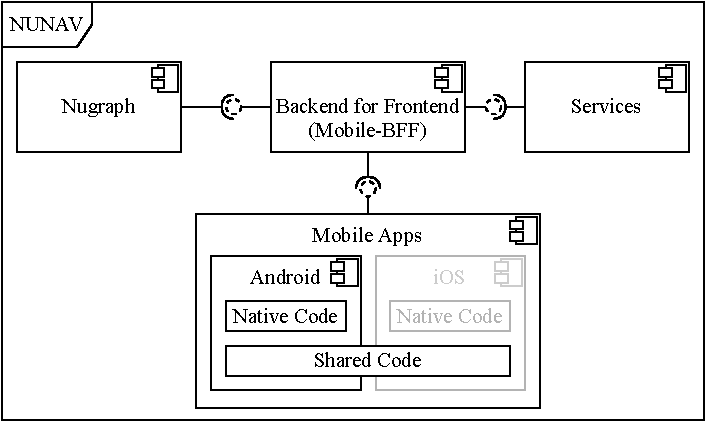
\includegraphics[width=\textwidth]{contents/06_model_evaluation/01_integration/res/nunav_architecture.pdf}
    \caption{Ausschnitt aus der NUNAV Software Architektur (UML-Komponenten-Diagramm)}
    \label{fig:nunav_software_architecture}
\end{figure}

\autoref{fig:nunav_software_architecture} stellt abstrakt alle für diese Arbeit relevanten Services der Infrastruktur dar. Wichtig ist dabei zum einen der Routingalgorithmus an sich (\textit{Nugraph}), welcher die Daten für die Navigation bereitstellt. Zum anderen ist die Mobile Anwendung von \textit{NUNAV Navigation} relevant, da dort Erklärungen integriert werden sollen. Außerdem gibt es für jede Client-Anwendung einen sogenannten BFF (\textit{Backend for Frontend}). Für diese Arbeit ist der \textit{Mobile BFF} relelvant. Dieser stellt die einzige Kommunikationsschnittstelle der Clients mit allen anderen Services der Infrastruktur dar. In der Regel wird die Kommunikation zwischen den Services bzw. Clients und dem BFF über REST
\footnote{\textit{Representational State Transfer} ist ein Paradigma zum Austausch von Daten über das HTTP-Protokoll.}
-Schnittstellen mit JSON
\footnote{\textit{JavaScript Object Notation} ist ein Datenformat, welches vor allem für Maschine-zu-Maschine-Kommunikation eingesetzt wird und Programmiersprachen unabhängig ist.}
als Übertragungsformat abgewickelt. 

\paragraph{Nugraph} \textit{Nugraph} ist der Gesamtbegriff in der Architektur für die Services, welche zum Routingalgorithmus gehören. Dieser berechnet auf der Basis eines prädiktiven Verkehrsmodells die individuell schnellste Route zwischen zwei Punkten. Dabei wird anhand von ca. 1,5 Millionen Verkehrsmessungen
 (z.B. \textit{Floating Car Data}\footnote{\textit{Floating Car Data} (FCD) sind mit Zeitstempeln versehene Geolokalisierungs- und Geschwindigkeitsdaten, die direkt von fahrenden Fahrzeugen erfasst werden})
 in der Minute der Verkehr auf der Route zum Zeitpunkt, zu dem Nutzer durch den Verkehr an einer Stelle beeinflusst werden, mithilfe von Künstlicher Intelligenz vorausgesagt. Alle Daten die zur Navigation (z.b. Verlauf und Geschwindigkeit auf der Route) benötigt werden kommen von diesem Teilsystem.

\paragraph{Backend for Frontend} Der in \autoref{fig:nunav_software_architecture} gezeigte \textit{Mobile-BFF} ist zum einen für die korrekte Weiterleitung von Anfragen an den richtigen Service zuständig. Darüber hinaus bereitet dieser auch Daten anderer Services für die Mobilen Apps auf oder konvertiert die verschiedenen Formate. Dabei werden zum Teil Daten mehrerer Services gebündelt oder neue Daten berechnet. 

\paragraph{Mobile Apps} Die mobilen Anwendungen für Smartphones bereiten zum einen die Daten der \textit{Micro-Services} für die Nutzer auf und zeigen sie diesen an. Zum anderen verarbeiten diese lokal die vom BFF bereitgestellte Routen und berechnen die Position auf dieser, zum Geben von Abbiege-Kommandos und Anzeigen des Routenverlaufs. Die \textit{Mobile Apps} werden für Android und iOS parallel in den jeweiligen vom Hersteller bereitgestellten Frameworks nativ entwickelt. Außerdem gibt es eine geteilte Code-Basis, welche Kotlin-Native\footnote{\textit{Kotlin-Native} ist eine Technologie zur Kompilierung von Kotlin-Code in Binärdaten für verschiedene Platformen und Prozessorarchitekturen.} als Technologie nutzt.

\bigskip

Die drei vorgestellten Systemteile sind jene, welche entweder Daten für Erklärungen liefern können, oder für die Auslieferung von Erklärungen an die \textit{End User} fungieren. Im Rahmen dieser Arbeit wurden dabei sowohl auf dem BFF, als auch in der Mobilanwendung für Android Änderungen vorgenommen. Außerdem wurden durch Änderungen von der Graphmasters GmbH in \textit{Nugraph} und einem weiteren Service vorgenommen, um benötigte Daten für die entwickleten Erklärungen zur Verfügung zu stellen.

\subsection{Ermittlung des Erklärungsbedarfs}
\label{sec:explanation_demand_generation}

Die Anwendung des Leitfadens zur Integration von Erklärungen ist in mehrere Teile gegliedert. In einem ersten Schritt wurden die existierenden Verständnisprobleme in NUNAV analysiert. Diese wurden aus verschiedenen Datenquellen der \textit{Graphmasters GmbH} zusammengefasst. Dazu zählen unter anderem mehrere Support-Kanäle.

Um diese Analyse anzureichern, wurde darauf aufbauend ein Workshop mit mehreren Mitarbeitern der \textit{Graphmasters GmbH} durchgeführt. Ergebnis diesen Workshops waren dann eine Aufstellung der Probleme, Ziele und Rohanforderungen für Erklärungen und Ideen zur Umsetzung. Auf Basis dieser Ergebnisse wurden dann im Rahmen dieser Arbeit die Anforderungen konkretisiert und in Designs für Erklärungen umgesetzt. Abschließend ist die technische Realisierung in \textit{NUNAV Navigation} erfolgt.

\subsubsection{User-Feedback-Analyse}

Für die initiale Analyse, welche Verständnisprobleme in \textit{NUNAV Navigation} bestehen, wurde zunächst manuell das Feedback, welches im Google Play Store und Apple App Store von Nutzern in Form von App-Reviews gegeben wurde, analysiert (ab Oktober 2020). Daraus sind Themengebiete abgeleitet worden, und die Anzahl der Reviews, die ein Themengebiet ansprechen, wurden gezählt. Aus insgesamt 304 Reviews konnten 46 identifiziert werden, aus denen klare Themen abgeleitet werden können. 33 dieser Review thematisieren Verständnisprobleme. Die Themen, die häufig vorkamen und für Erklärbarkeit relevant sind, sind in \autoref{sec:appendix_literature_research} aufgelistet. Dabei wurde als Hauptproblem ein zu geringes Verständnis für den kollaborativen Routing-Algorithmus identifiziert. Allein fünf der 16 Reviews, aus denen sich dies ableiten lässt, bemängeln, dass NUNAV keine Alternativrouten vorschlägt. Dies weist darauf hin, dass nicht klar ist, dass das System des Verteilens der Nutzer auf die vorhandene Verkehrsinfrastruktur nur möglich ist, wenn die Nutzer den vorgeschlagenen Routen folgen und keine Alternativen nehmen.

Außerdem gibt es Hilfe-Artikel, die über einen \textit{Hilfe-Center} der \textit{Graphmasters}-Webseite erreichbar sind\footnote{\url{https://support.graphmasters.net/}, besucht: 01.10.21}. Dabei wurden die Klickzahlen mit den Review-Anzahlen verglichen, welche vom Verhältnis her ähnlich der Anzahlen an Reviews ist.

Aus den Reviews und Hilfe-Center-Artikeln wurden dann erste Themen beziehungsweise Nutzerfragen abgeleitet und mit dem Team \glqq Solution Experts\grqq{} von \textit{Graphmasters} diskutiert. Das Team ist für die Betreuung von Kunden und die Bearbeitung von Feedback zuständig. Die Ergebnisse sind in \autoref{tab:06_model_evaluation_explicit_questions} zu sehen.

\begin{table}[htb!]
    \begin{tabular}{p{.3\textwidth}p{.66\textwidth}}
        \hline
        Thema         & Fragen \\
        \toprule
        Kollaboratives Routing  & Was ist / wie funktioniert kollaboratives Routing? \\
        &  Warum brauche ich eine ständige Internetverbindung? \\
        &  Wieso werden in NUNAV keine Standardrouten angezeigt?\\
        \tablerowspacing
        Navigation              & Warum wird diese Route / der Umweg genommen? \\
        & Warum sind die Routen bei NUNAV länger? \\
        & Warum ist die Position ungenau? \\
        \tablerowspacing
        Vertrauen in das System & Woher kommen die Verkehrs-/ Sperrungsdaten? \\
        & Was passiert mit meinen Daten? \\
        & Wofür benötige ich Ortungsdienste beim App-Start? \\
        & Kann die Güte der Route nicht bewerten? \\
        \tablerowspacing
        Funktionen   & Was zeigt die Rainbow-Route an? \\
        & Wie kann ich eine Sperrung melden? \\
        & Wie kann ich mein Ziel in NUNAV eingeben? \\
        & Wie kann ich Favoriten anlegen? \\
        \toprule
    \end{tabular}
\caption{Anzahl der Reviews im Google Play Store und Apple App Store mit mehrfach vorkommenden Themen}
\label{tab:06_model_evaluation_explicit_questions}
\end{table}

\bigskip

Auf Basis dieser ersten Ergebnisse wurde im Anschluss ein Workshop mit mehreren \textit{Graphmasters}-Mitarbeitern durchgeführt.

\subsubsection{Workshop zur Integration von Erklärungen}

Zum Festlegen der Ziele und Anforderungen an die Erklärungen sowie zum Sammeln erster Umsetzungsideen, wurde ein interdisziplinärer Workshop mit Frontend-Entwicklern, \glqq Solution Experts\grqq{} und einem Produktmanager bei \textit{Graphmasters} durchgeführt. Außerdem sollten Metriken gefunden werden, welche zur Überprüfung der Ziele verwendet werden können. Durch die direkte Anwendung des entwickelten Leitfadens im Workshop konnten außerdem Beobachtungen darüber, wie dieser eingesetzt wird, gesammelt werden. Dies war allerdings nicht Kern des Workshops. 

Nach der initialen Vorstellung von Erklärbarkeit, dem Leitfaden für die Integration von Erklärungen sowie den Ergebnissen aus der User-Feedback-Analyse hat sich der Workshop an dem Aufbau des Modells für Erklärungen orientiert. Folglich wurden zuerst Informationen zu möglichen Nutzern (\textit{Context}), dann Ziele (\textit{Objectives}) und deren Umsetzungsmöglichkeiten (\textit{Characteristics}) und schließlich die Evaluationsmöglichkeiten besprochen (\textit{Evaluation}). Auch wenn der Workshop so geplant war, dass die einzelnen Aspekte nacheinander abgearbeitet werden, hat sich ergeben, dass die Ziele und deren Umsetzung gleichzeitig behandelt wurden. Grund dafür war, dass beim Aufstellen der Ziele und Rohanforderungen bereits die Umsetzbarkeit im Rahmen dieser Arbeit diskutiert wurde. Einige Fragen der Machbarkeit sind allerdings ungeklärt geblieben, da hierfür Wissen von den Entwicklern des Routing-Algorithmus benötigt wurde. Explizit ging es um die Frage, welche Daten für bestimmte Erklärungen überhaupt zur Verfügung gestellt werden können. Ein detailliertes Ergebnisprotokoll des Workshops ist in \autoref{sec:appendix_workshop_protocol} zu finden.

\newpage

Aus den Ergebnissen des Workshops wurden dann iterativ und in Rücksprache mit verschiedenen Teilnehmern des Workshops Personas, die konkreten Anforderungen sowie die finalen Erklärungen, die in \textit{NUNAV Navigation} integriert werden sollten, entwickelt.

\subsection{Personas von NUNAV-Nutzern}
\label{sec:06_model_evaluation:personas}

Um die Interpreation der Rohanforderungen aus dem durchgeführten Workshop besser interpretieren zu können, wurden Personas für typische NUNAV-Nutzergruppen abgeleitet. Graphmasters hat zwar kein genaues Bild, darüber welche Nutzertypen \textit{NUNAV Navigation} nutzen, aus einzelnen Nutzer-Gesprächen aus der Vergangenheit haben sich allerdings zwei Gruppen herauskristalisiert, die klar benennbar sind.

\begin{wrapfigure}{o}{0.33\textwidth}
    \vspace{-\intextsep}
    \centering
    
\includegraphics[width=0.3\textwidth]{contents/06_model_evaluation/01_integration/res/persona_picture_michael.png}
    \caption{Michael -\\Lizensiert bei Shutterstock Nr. 602783837}
\end{wrapfigure}

\paragraph{Vielfahrer} Michael, 34 Jahre alt, arbeitet als Unternehmensberater in einem großen Beratungsunternehmen. Er hat Betriebswirtschaftleere studiert und ist seit dem Studium in der Firma.

Er wohnt mit seiner Frau und einer Tochter in der Vorstadt und muss jeden morgen zur Hauptverkehrsszeit in die Stadt fahren, um in sein Büro zu kommen. Dadurch steht er nahezu täglich im Stau auf dem Weg zur Arbeit. Die öffentlichen Verkehrsmittel kommen für ihn nicht in Frage, da er mit ihnen mehr als doppelt so lange bräuchte. Auch zu Vortortterminen beim Kunden fährt er ungefähr einmal pro Woche. Dabei interessiert ihn vor allem, wie hoch das Verkehrsaufkommen zu dem Zeitpunkt auf der Strecke ist.

Lange Zeit hat er das in sein Auto integrierte Navigationssystem verwendet, das aber nur vereinzelt auf Staus reagiert hat und ihn jeden Tag auf der gleichen Strecke zur Arbeit geschickt hat, wenn nicht ein besonderes Ereignis wie Unfälle oder Sperrungen auf der Strecke waren.

Michael hat ein modernes Dienst-Smartphone mit Android und ist generell technik interessiert. Zwischendurch hat er die auf seinem Smartphone vorinstallierte Navigations-App verwendet, da diese immer aktuellen Verkehr anzeigen kann. Diese leitetete ihn zum Teil aus dem Stau des Berufsverkehrs raus, in dem er stand. Er hat aber meist ähnlich lange zur Arbeit gebraucht wie im Stau. Außerdem achtet Michael darauf, was mit seinen Daten passiert und da ist er sich bei dem Anbieter nicht sehr sicher, wie anonym diese verarbeitet werden.

Seit einigen Tagen verwendet er die Navigations-App \text{NUNAV Navigation}, die verspricht ihn jeden Tag auf dem schnellsten Weg zur Arbeit zu bringen. Die App schlägt ihm ab und zu seiner Meinung nach \glqq komische\grqq{} Routen vor. Anfangs hat er sich dann nicht an diese gehalten. Dann hat er die Alternativen ausprobiert. Tatsächlich war er etwas schneller als sonst auf dem Weg zur Arbeit. Er ist aber immer noch skeptisch, da er die vorgeschlagenen Routen nicht immer versteht und bei sich bei Umwegen immer noch auf seine Intuition verlässt.

\bigbreak

\begin{wrapfigure}{o}{0.33\textwidth}
    \vspace{-\intextsep}
    \centering
    
\includegraphics[width=0.3\textwidth]{contents/06_model_evaluation/01_integration/res/persona_picture_ayla.png}
    \caption{Ayla -\\Lizensiert bei Shutterstock Nr. 1433736386}
\end{wrapfigure}

\paragraph{Erstnutzer} Ayla ist 23 Jahre alt und studiert aktuell Mathematik im 7. Bachelorsemester. Sie wohnt in einem Studentenwohnheim und fährt jeden Tag mit der Bahn zur Universität. Sie kommt ursprünglich aus einem Dorf ca. 300~km entfernt besucht ihre Eltern dort mindestens dreimal im Monat am Wochenende. Dafür hat sie ein Auto, da sie mit ihrem Semesterticket nicht bis in die Heimat fahren kann.

% 2. Event-Fahrer (Erste Nutzung, kennt den kollaborativen Ansatz nicht.) Lorem ipsum dolor sit amet, consetetur sadipscing elitr, sed diam nonumy eirmod tempor invidunt ut labore et dolore magna aliquyam erat, sed diam voluptua. At vero eos et accusam et justo duo dolores et ea rebum. Stet clita kasd gubergren, no sea takimata sanctus est Lorem ipsum dolor sit amet. Lorem ipsum dolor sit amet, consetetur sadipscing elitr, sed diam nonumy eirmod tempor invidunt ut labore et dolore magna aliquyam erat, sed diam voluptua. At vero eos et accusam et justo duo dolores et ea rebum. Stet clita kasd gubergren, no sea takimata sanctus est Lorem ipsum dolor sit amet.

% Lorem ipsum dolor sit amet, consetetur sadipscing elitr, sed diam nonumy eirmod tempor invidunt ut labore et dolore magna aliquyam erat, sed diam voluptua. At vero eos et accusam et justo duo dolores et ea rebum. Stet clita kasd gubergren, no sea takimata sanctus est Lorem ipsum dolor sit amet. Lorem ipsum dolor sit amet, consetetur sadipscing elitr, sed diam nonumy eirmod tempor invidunt ut labore et dolore magna aliquyam erat, sed diam voluptua. At vero eos et accusam et justo duo dolores et ea rebum. Stet clita kasd gubergren, no sea takimata sanctus est Lo

\subsection{Anforderungen der Erklärungen}

Mithilfe der Rohanforderungen und Ziele aus dem Workshop sowie den erstellten Personas können sowohl funktionale als auch nicht-funktionale Anforderungen für Erklärungen in NUNAV entwickelt werden

\subsubsection{Nicht-Funktionale Anforderungen}

% \cite{kohl_explainability_2019} gives a good overview to the requirement analysis for Explainability as an NFR

Als Methode zum Ableiten der konkreten NFRs wurde das Aufstellen eines Qualitätsmodells gewählt \cite{schneider2012abenteuer}. Das Modell ist in \autoref{fig:nunav_explanation_quality_model} dargestellt. Bei der Erstellung wurde iterativ Rücksprache mit den verschiedenen Teilnehmern des Workshops gehalten. Als Basis für die Qualitätsziele wurden die in dem Modell für Erklärungen unter \textit{Objectives} aufgeführten Ziele verwendet. Die Endfassung der Anforderungen wurde schlussendlich vom Teamleiter des \glqq Mobile Application\grqq{}-Teams abgesegenet.

Es hat sich allerdings herausgestellt, dass das Aufstellen solch konkreter Anforderungen nicht der Arbeitsweise von Graphmasters entspricht. In den Rücksprachen wurde klar, dass die Ziele normalerweise deutlich abstrakter gehalten werden. Für eine Evaluation der Integration von Erklärungen im Rahmen dieser Arbeit werden die konkreten Anforderungen zur Prüfung allerdings benötigt.

\begin{figure}[htb!]
    \centering
    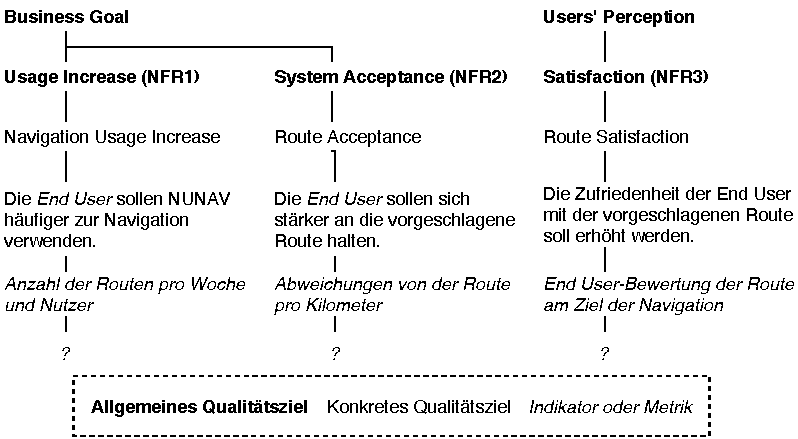
\includegraphics[width=\textwidth]{contents/06_model_evaluation/01_integration/res/quality_model.pdf}
    \caption{Qualitätsmodell für die Integration von Erklärungen in NUNAV Navigation}
    \label{fig:nunav_explanation_quality_model}
\end{figure}

In \autoref{fig:nunav_explanation_quality_model} ist zu erkennen, dass für Graphmasters im Allgemeinen die Erhöhung der Nutzung und die Akzeptanz des Systems im Vordergrund stehen. Bei der Nutzung ist für Graphmasters die interessanteste Metrik die Anzahl der aktiven Nutzer. Da sich eine Messung von Veränderungen dieser durch die Integration von Erklärungen allerdings nicht über einen kurzen Zeitraum messen lässt, wurde  als Metrik die Anzahl der Routen pro Nutzer und Woche vorgeschlagen und schließlich auch durch Graphmasters bestätigt. Für die Akzeptanz des Systems ist ein Ziel, dass sich die \textit{End User} möglichst viel an die vorgeschlagene Route halten. Als Metrik wurde hierfür die Anzahl der Abweichungen von der Route pro Kilometer verwendet.

Ein weiteres wichtiges Ziel von Graphmasters ist die Zufriedenheit der \textit{End User} mit den Routen. Hierfür bestand bereits vor dem Beginn dieser Arbeit eine Metrik. \textit{End User} können bei Erreichen des Ziels einer Navigation auf einer Skala mit ein bis fünf Sternen angeben, wie zufrieden sie insgesamt mit der Route waren. Bis dato wurde diese Metrik allerdings noch nicht systematisch ausgewertet.

Für alle Metriken fällt auf, dass in \autoref{fig:nunav_explanation_quality_model} keine Sollwerte definiert sind. Aus den Gesprächen hat sich ergeben, dass für Graphmasters erstens nicht wichtig ist, um wie viel die verschiedenen Metriken sich verbessern, solange mit der Integration von Erklärungen eine Besserung eintritt. Außerdem ist sind keine Basiswerte vorhanden, auf die man sich beziehen kann. Aus diesem Grund wurden die konkreten Anforderungen in Bezug auf signifikante Unterschiede formuliert. Die Formulierungen orientieren sich dabei an gängigen Vorlagen, enthalten allerdings nicht die in den Vorlagen geforderten Sollwerte \cite{rajnish2010quality, wiegers1999writing, alexander2002writing}:

\begin{enumerate}
    \item [NFR1] Die Anzahl der gefahrenen Routen mit \textit{NUNAV Navigation} pro Nutzer und Woche soll signifikant messbar erhöht werden.
    \item [NFR2] Die durchschnittliche Anzahl der Abweichungen der Nutzer pro Kilometer von der durch \textit{NUNAV Navigation} vorgeschlagenen Route soll signifikant messbar verkleinert werden.
    \item [NFR3] Die durchschnittliche Bewertung der Route am Ende der Navigation in \textit{NUNAV Navigation} soll signifikant messbar erhöht werden.
\end{enumerate}

\subsubsection{Funktionale Anforderungen}

In diesem konkreten Fall stand die Integration von Erklärungen als Lösungsansatz zum Erreichen der Ziele bereits fest. Daher wurden die \textit{Explanation Goals} aus dem Modell für Erklärungen ausgewählt, welche in Erklärungen umgesetzt werden sollten. Dabei steht vor allem auch die Frage im Raum, welche Aspekte genau erklärt werden müssen \cite{kohl_explainability_2019}.

Ein Ergebnis des durchgeführten Workshops war die Verständnisprobleme der Nutzer, welche durch Erklärungen gelöst werden sollen und erste Umsetzungsideen. Aus diesen beiden Punkten konnten \textit{Transparency} und \textit{Scrutability} als Ziele für die Integration von Erklärungen abgeleitet werden.
% Da die vorherigen Qualitätsanforderungen sehr Allgemein auf \textit{NUNAV Navigation} bezogen sind, ist das Ziel, dass sich alle integrierten Erklärungen positiv auf die Qualitätsziele auswirken.

Auch die Konkretisierung der funktionalen Anforderungen ist iterativ erfolgt. Eine Herausforderung dabei war vor allem, dass Graphmasters in der Regel keine konkreten Anforderungen formuliert, sondern direkt anhand von Ideen Mockups erstellt und dann iterativ mehrere Prototypen entwickelt.

Für die funktionalen Anforderungen wurde ein Zielbaum ähnlich zu Qualitätsmodellen aufgestellt, in dem die Konkretisierungsschritte zu sehen sind. \autoref{fig:nunav_explanation_functional_model} stellt diesen dar.

\begin{figure}[htb!]
    \centering
    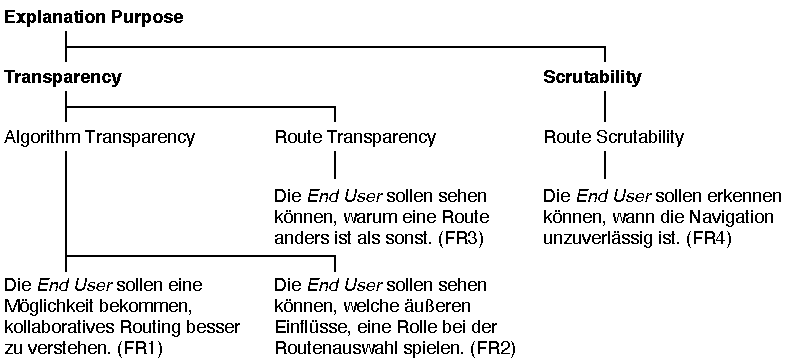
\includegraphics[]{contents/06_model_evaluation/01_integration/res/functional_model.pdf}
    \caption{Konkretisierungsschritte bei der Entwicklung der funktionalen Anforderungen an Erklärungen in \textit{NUNAV Navigation}}
    \label{fig:nunav_explanation_functional_model}
\end{figure}

Aus den Konkretisierungsschritten (siehe \autoref{fig:nunav_explanation_functional_model}) wurden schlussendlich folgende funktionalen Anforderungen abgeleitet:
% . Die in der Abbildung als FR1 abgebildete unkonkrete Anforderung wurde im letzten Konkretisierungsschritt in zwei Anfroderungen (FR1.1, FR1.2) aufgeteilt.

\begin{enumerate}
    \item [FR1] \textit{NUNAV Navigation} muss den \textit{End Usern} die Möglichkeit bieten, auf eine Erklärung zuzugreifen zu können, die den kollaborativen Routingalgorithmus erklärt.
    \item [FR2] \textit{NUNAV Navigation} muss den \textit{End Usern} die Möglichkeit bieten, abzurufen, welche Informationen zu Verkehrsereignissen (z.B. Verkehrsfluss, Sperrungen, Baustellen, Staus) in den Algorithmus einfließen.
    \item [FR3] \textit{NUNAV Navigation} muss den \textit{End Usern} während der Navigation Informationen zum Verkehrsgeschehen auf der aktuellen Route liefern.
    \item [FR4] Wenn die Genauigkeit der Positionierung unzuverlässig ist, muss \textit{NUNAV Navigation} den \textit{End Usern} anzeigen, dass die Positionierung aktuell nicht zuverlässig ist.
\end{enumerate}

Auf Basis dieser Anforderungen wurden dann Erklärungen für die Integration in \textit{NUNAV Navigation} entwickelt.

\subsection{Design der Erklärungen}

Das Gestalten der Erklärungen ist mit mehreren Design-Mockups umgesetzt worden. Grundsätzlich ist für die funktionalen Anforderungen 1-4 jeweils ein Erklärungstyp entstanden. Wie aus Protokoll des durchgeführten Workshops zu entnehmen ist, wurden bereits in diesem einige Ideen für Erklärungen auf Basis der Vorschläge zur Umsetzung von Erklärungen aus dem Modell für Erklärungen entwickelt.

Außerdem wurden bei der Umsetzung die Zusammenhänge zwischen den Eigenschaften von Erklärungen auf Qualitätsaspekte sowie die Heuristiken für das Design von Erklärungen beachetet. Insbesondere wurde darauf geachtet, dass die Erklärungen dezent sind, sodass sie möglichst keinen negativen Einfluss auf die \textit{Usability} haben. Längere Erklärungen wurden nur optional eingesetzt. Auch wurde wie aus dem Leitfaden hervorgeht, versucht für eine Information möglichst hybride Stile zu nutzen, sodass die \textit{End User} diese auf mehrere Weisen erfassen können.

Da eine weitere wichtige Empfehlung die \textit{Context Sensitivity} von Erklärungen betrifft, wird hier kurz auf den \textit{Context} eingegangen. Die \textit{End User} wurden bereits zurvor beschrieben (siehe \autoref{sec:06_model_evaluation:personas}). Grundsätzlich kann im \text{Context} von Navigationsanwendungen zwischen zwei verschiedenen Situationen unterschieden werden. Die erste ist die Nutzung von \textit{NUNAV Navigation} vor der aktiven Navigation. Dies beinhaltet das Auswählen des Ziels, eine Routenübersicht, sowie dann die Möglichkeit des startens der Navigation. Hier haben die \textit{End User} keinen Zeitdruck und können sich auf die Interkation mit der Applikation konzentrieren. Trotz dessen wurden die Erklärungen so entwickelt, dass diese von den \textit{End Usern} wie von \citeauthor{chazette_end-users_nodate} sowie \citeauthor{wang_integration_2020} vorgeschlagen, optional angefordert werden müssen \cite{chazette_end-users_nodate,wang_integration_2020}. Folglich wurden für die Anfroderungen FR1 und FR2 in diesem \textit{Context} umgesetzt. Grund dafür ist, dass die Informationsmenge zur Erklärung des Routingalgorithmus und der dazugehörigen Daten so groß ist, dass eine Integration in die zweite mögliche Situation nicht ohne Beeinflussung der Nutzerperformanz möglich wäre.

Die zweite Situation ist die aktive Navigation. Während dieser sollten die \textit{End User} zu wenig wie möglich abgelenkt werden, da sie der vollen Konzentration auf die Straße bedürfen. Daher sind alle Erklärungen, die während der Navigation den \textit{End Usern} zur Verfügung gestellt werden entgegen der Empfehlung für Interaktionen mit Erklärungen ohne eine Manipulationsmöglichkeit durch die \textit{End User} gestaltet.

Die vier entwickelten Erklärungstypen werden im Folgenden im Detail vorgestellt.

% Grafiken von eingehendem Datenstrom und ausgehenden Datenstrom.
% explain \textit{Affordance}

\subsubsection{Kollaboratives Routing}
\label{sec:user_count_definition}

\paragraph{[FR1]} NUNAV muss den \textit{End Usern} die Möglichkeit bieten, auf eine Erklärung zuzugreifen zu können, die den Routingalgorithmus erklärt.

\bigskip

Wie bereits erläutert ist der Kerngedanke des \textit{NUNAV}-Routingalgorithmus, dass jeder \textit{End User} eine individuell schnellste Route erhält und dabei nicht zwangsweise Hauptverkehrsstraßen nutzt. Folglich ist für diese erste Anforderung eine Erklärung entworfen worden, die das Kollaborative Routing erklärt.

Wie bei genauerem Einblick in das Feedback von \textit{End Usern} auffällt, ist eines der Grundprobleme, dass ihnen das Verständnis fehlt, dass sie vernetzt mit anderen Nutzern von \textit{NUNAV} kollaborativ navigiert werden. Da dies einer der Hauptunterschiede zu anderen Navigationsanbietern ist, sind Erklärungen die diesen Punkt betreffen vor allem für Erstnutzer wie Ayla wichtig. Um den Nutzern einen Einblick in diese Abhängigkeit von anderen Verkehrsteilnehmern zu geben, wird die aktuelle Anzahl der Nutzer, welche sich in einem Bereich, der die eigene Route beeinflusst, befinden angezeigt. Diese Berechnung dieser Zahl ist eine Annäherung, da sich nicht genau bestimmen lässt, welche Fahrzeuge auf der Straße einen realen Einfluss auf die eigene Navigation haben. Die Annäherung wurde allerdings als ausreichend befunden da, wie im Leitfaden beschrieben wird, die Richtigkeit der Erklärung keinen Einfluss auf die \textit{Transparency} hat, welche Ziel dieser Anforderung ist. In einem ersten Entwurf wurden alle aktiven Nutzer im System als Zahl angenommen. Dies wurde allerdings verworfen, da Nutzer aus dieser Zahl wenig Informationen über den unmittelbaren Einfluss auf für eigene Navigation bekommen.

Die Anzahl der Nutzer wurde von einem Backend-Team bei Graphmasters zur Verfügung gestellt, die restliche Umsetzung in \textbf{BFF} und App ist im Rahmen dieser Arbeit erfolgt. Für die Anzeige der Nutzerzahl wurden verschiedene Positionen im User Interface ausprobiert, wie in \autoref{fig:prototype_collaborative_routing} zu erkennen ist. Für die finale Version ist die Entschiedung gefallen, da an dieser Stelle bereits andere Informationen als sogenanntes \textit{Growl} angezeigt werden und diese Stelle zur Anzeige kurzer Informationen somit im Rahmen der \textit{Usabiltiy} bereits erfolgreich ohne negatives Feedback genutzt wird. Das \textit{Growl} ist in den Screenshots (a) und (b) der Abbildung rot umrahmt.

Eine Erklärung des Algorithmus ist in zwei verschiedenen Granulariätsstufen umgesetzt worden. Tippen \textit{End User} auf das \textit{Growl} mit der Anzahl der Nutzer gelangen sie zu einer kurzen Erklärung (siehe \autoref{fig:prototype_collaborative_routing}, (c)). Ursprünglich war der Text \glqq In den letzten 15 Minuten haben wir anonyme Verkehrsdaten von x Nutzern in deiner Umgebung erhalten\grqq{}. Nachdem zu diesem Text intern bei Graphmasters das Feedback kam, dass dieser zu technisch bzw. datengetrieben ist, wurde dieser so geändert, dass der direkte Einfluss auf die \textit{End User} klar wird (siehe \autoref{fig:prototype_collaborative_routing}, (c)).

Als weitere Erklärungsmöglichkeit können die \textit{End User} mittels \glqq Mehr erfahren\grqq{} zu dem entsprechenden Hilfe-Center-Artikel springen (siehe \autoref{sec:help_center_collaboratrive_routing}). Eine Verknüfung aus der App heraus direkt zum Hilfe-Center gab es an dieser Stelle noch nicht.

\begin{figure}[htb!]
    \centering
    \subfloat[1. Prototyp zur Positionierung der Nutzerzahl]
    {
        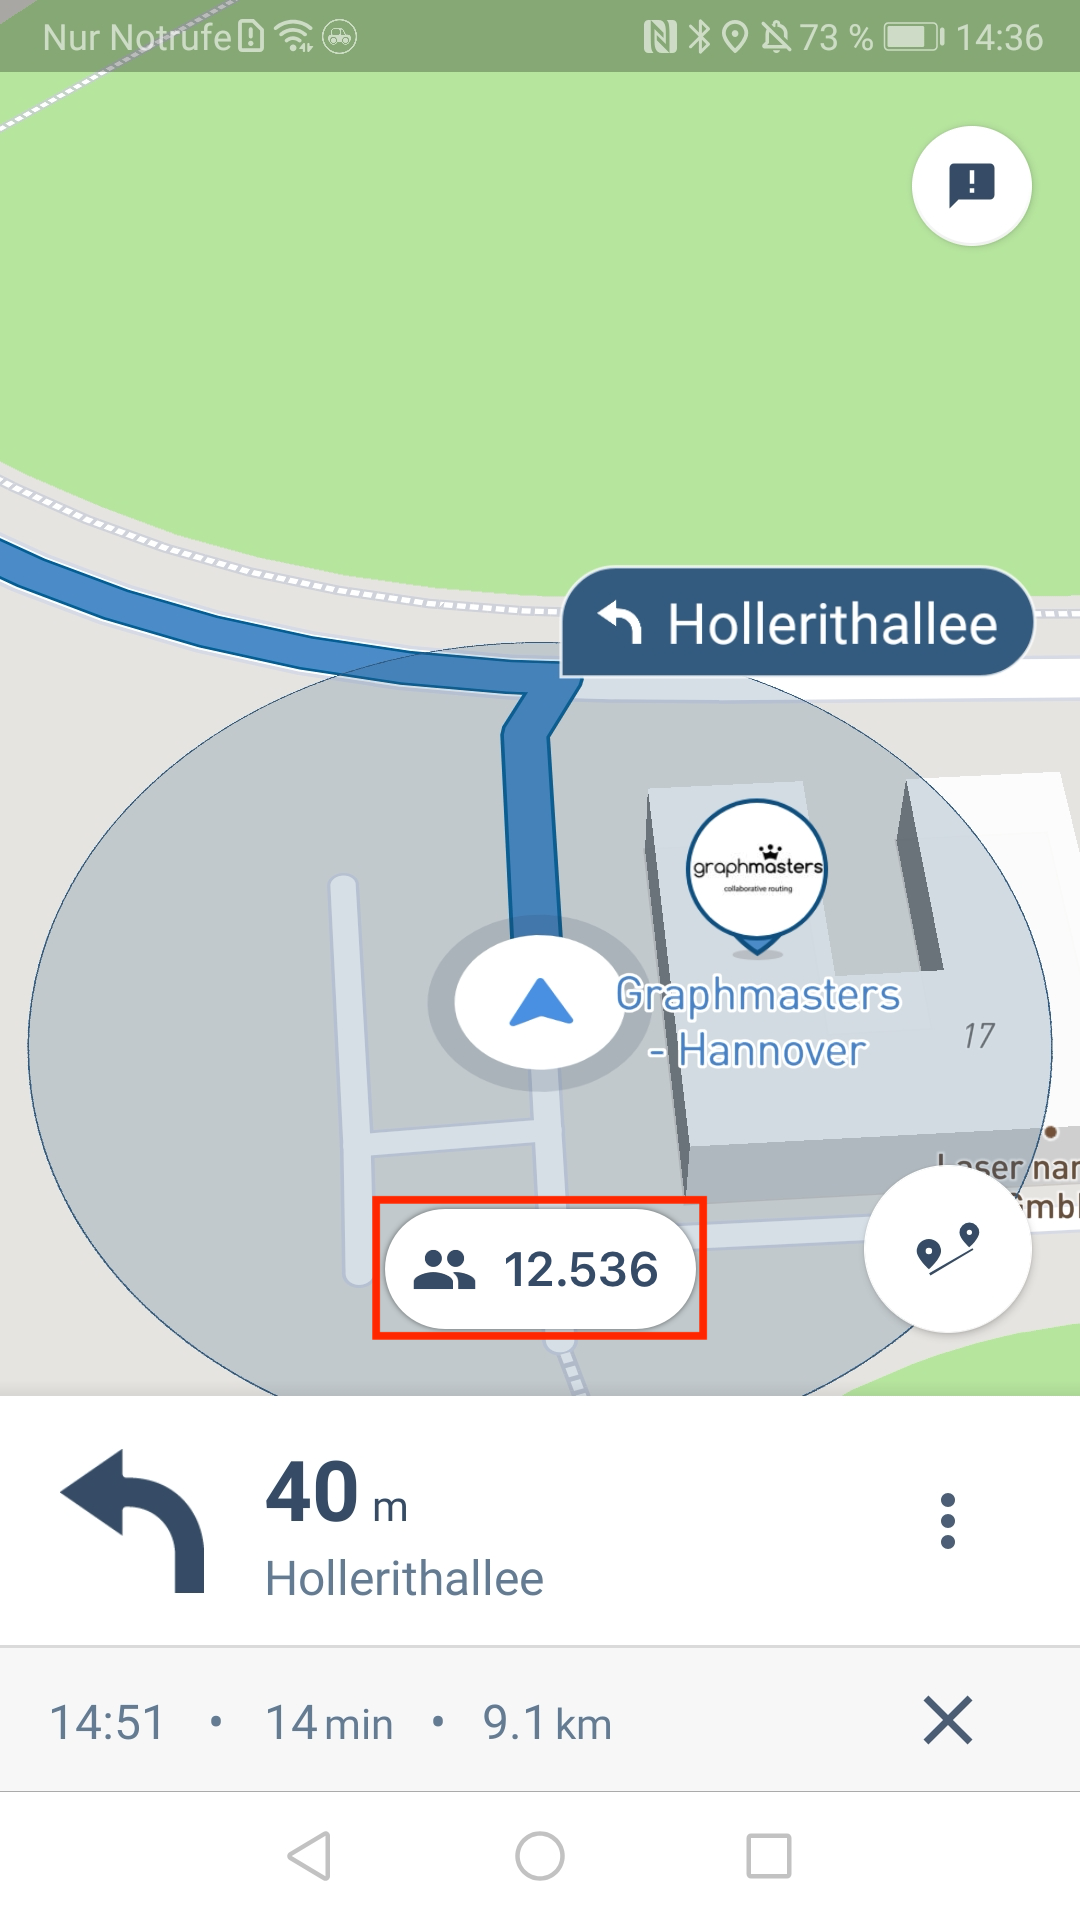
\includegraphics[width=.27\linewidth]{contents/06_model_evaluation/01_integration/res/01_collaborative_routing/prototype_1.png}
    }
    \hspace{.055\linewidth}
    \subfloat[Finales Design der Positionierung der Nutzerzahl]
    {
        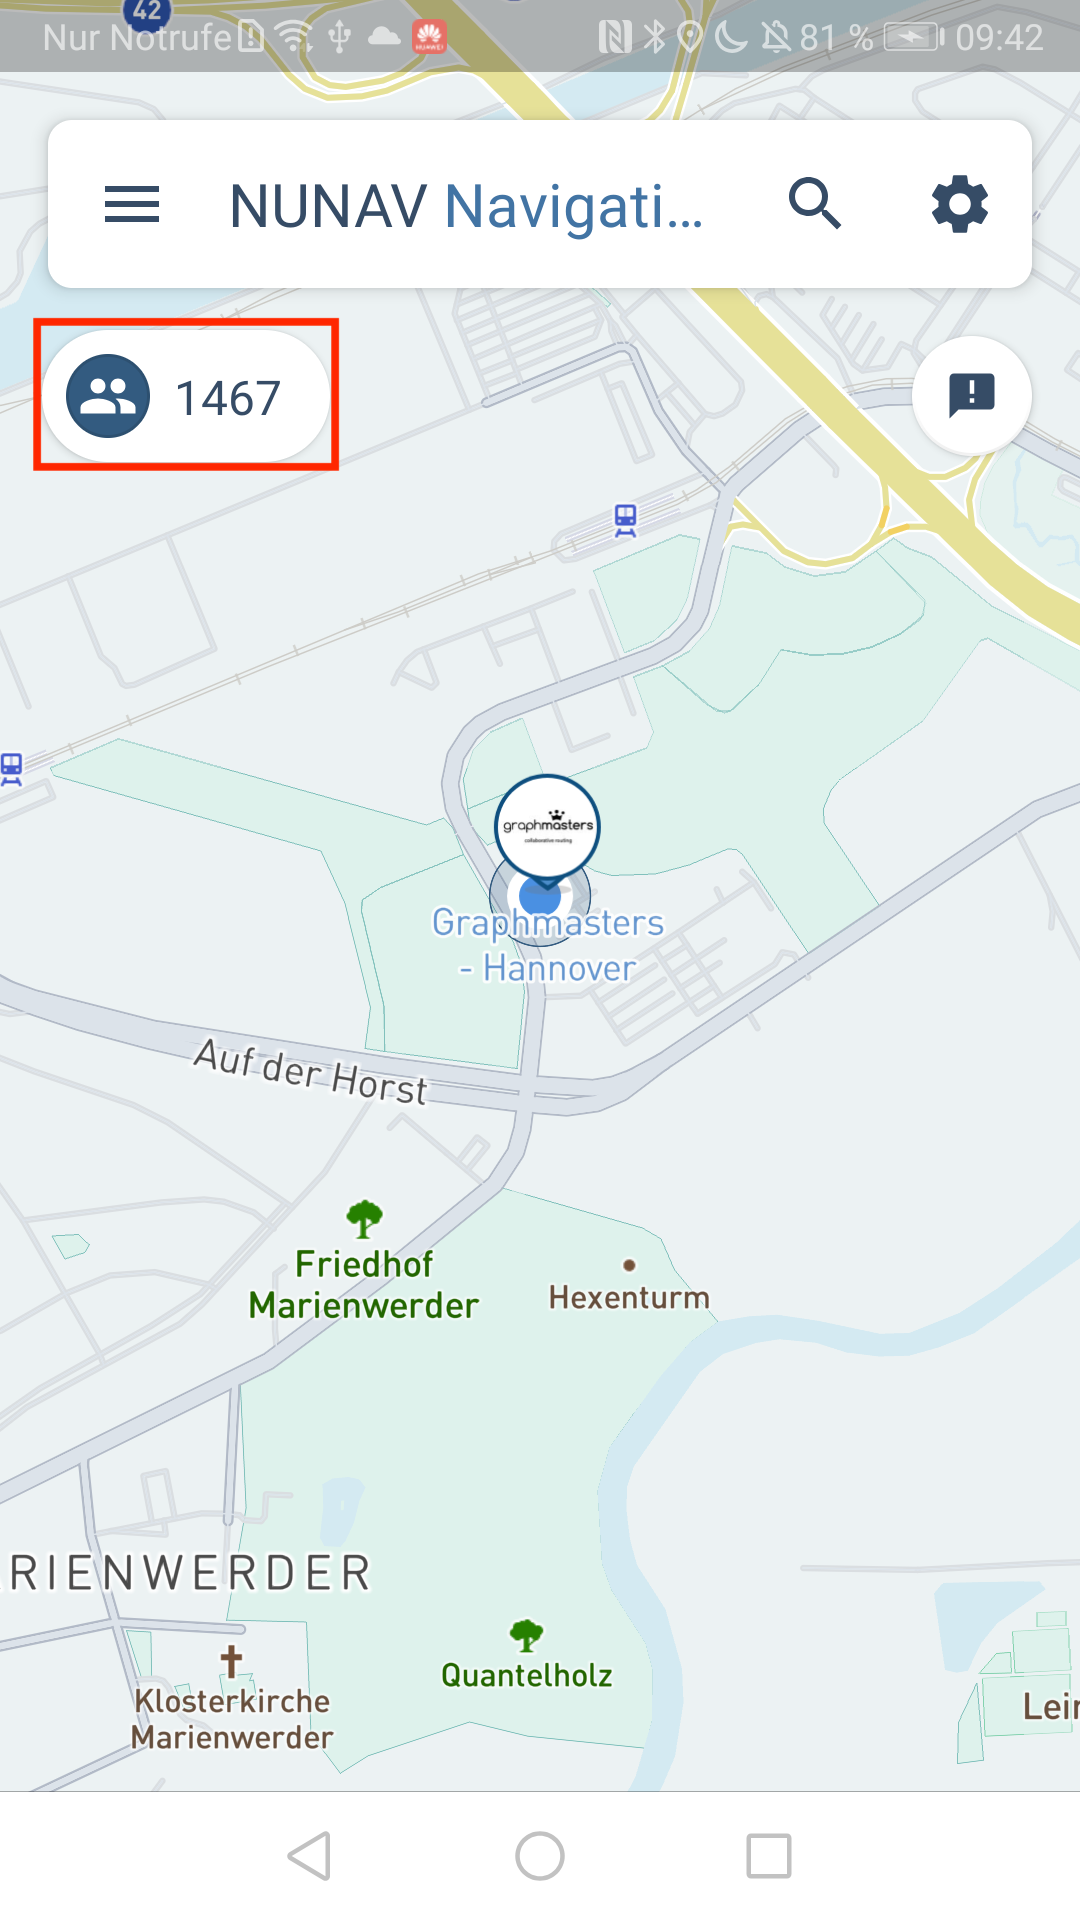
\includegraphics[width=.27\linewidth]{contents/06_model_evaluation/01_integration/res/01_collaborative_routing/final_1.png}
    }
    \hspace{.055\linewidth}
    \subfloat[Finales Design der kurzen Erklärung zum kollaborativen Routing]
    {
        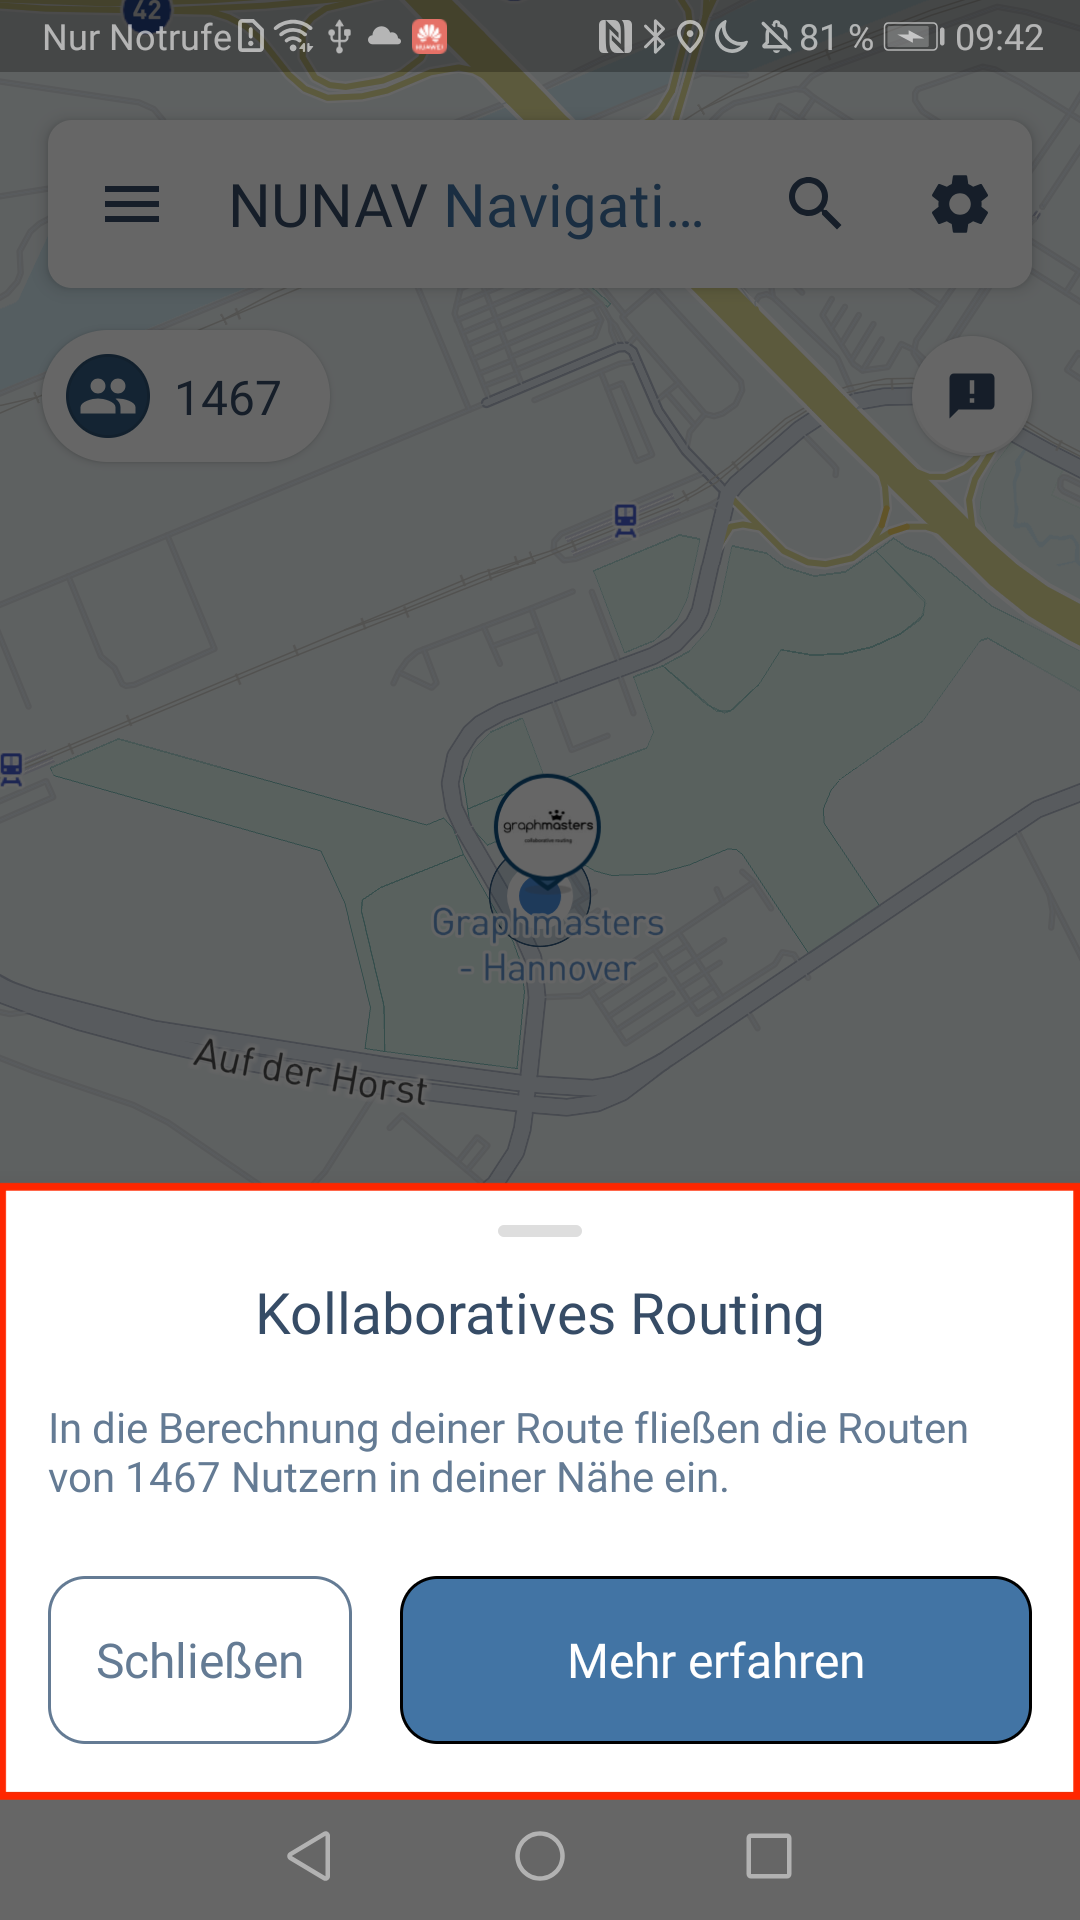
\includegraphics[width=.27\linewidth]{contents/06_model_evaluation/01_integration/res/01_collaborative_routing/final_2.png}
    }
    \caption{Prototyp und finale Designs für die Erklärung zum kollaborativem Routing}
    \label{fig:prototype_collaborative_routing}
\end{figure}

\subsubsection{Einflüsse auf die Routenberechnung}

\paragraph{[FR2]} \textit{NUNAV Navigation} muss den \textit{End Usern} die Möglichkeit bieten, abzurufen, welche Informationen zu Verkehrsereignissen (z.B. Verkehrsfluss, Sperrungen, Baustellen, Staus) in den Algorithmus einfließen.

\bigskip

Auf der Karte, welche das Hauptinteraktionselement von \textit{NUNAV Navigation} darstellt, sind Sperrungen, Baustellen und Staus bereits eingezeichnet. Wie aus dem Nutzerfeedback hervorgeht reichen diese \textit{Context}-Informationen allerdings für das Verständnis der \textit{End User} nicht aus. Daher wurde ein neuer Hilfe-Center-Artikel im Rahmen dieser Arbeit zu diesem Thema angelegt (siehe \autoref{sec:help_center_routing_data}). Dieser Artikel ist für Nutzer geeignet, welche NUNAV zum ersten Mal wie Ayla oder noch nicht lange wie Michael verwenden. So können sie sich anhand der Daten auf der Karte im Anschluss an das Lesen des Artikels die verschiedenen Routen besser erklären.

Dieser Beitrag wurde ebenfalls vor dem Start der Navigation erreichbar gemacht. Um die Standardkartenansicht nicht durch mehrere Möglichkeiten zum Aufrufen von Hilfe-Center-Artikeln zu überladen, wurde die Möglichkeit, zu dieser Erklörung zu gelangen, in die Routen-Vorschau integriert. Auch für diese wurden mehrere Prototypen erstellt, wobei bei der finalen Entscheidung darauf geachtet wurde, dass die Aufrufmöglichkeit nicht zu viel Platz einnimmt und der Text neugierig macht. Die verschiedenen Prototypen sind in \autoref{fig:prototype_routing_explanation} zu sehen.

\begin{figure}[htb!]
    \centering
    \subfloat[1. Prototyp zur Positionierung des Aufrufs der Erklärung]
    {
        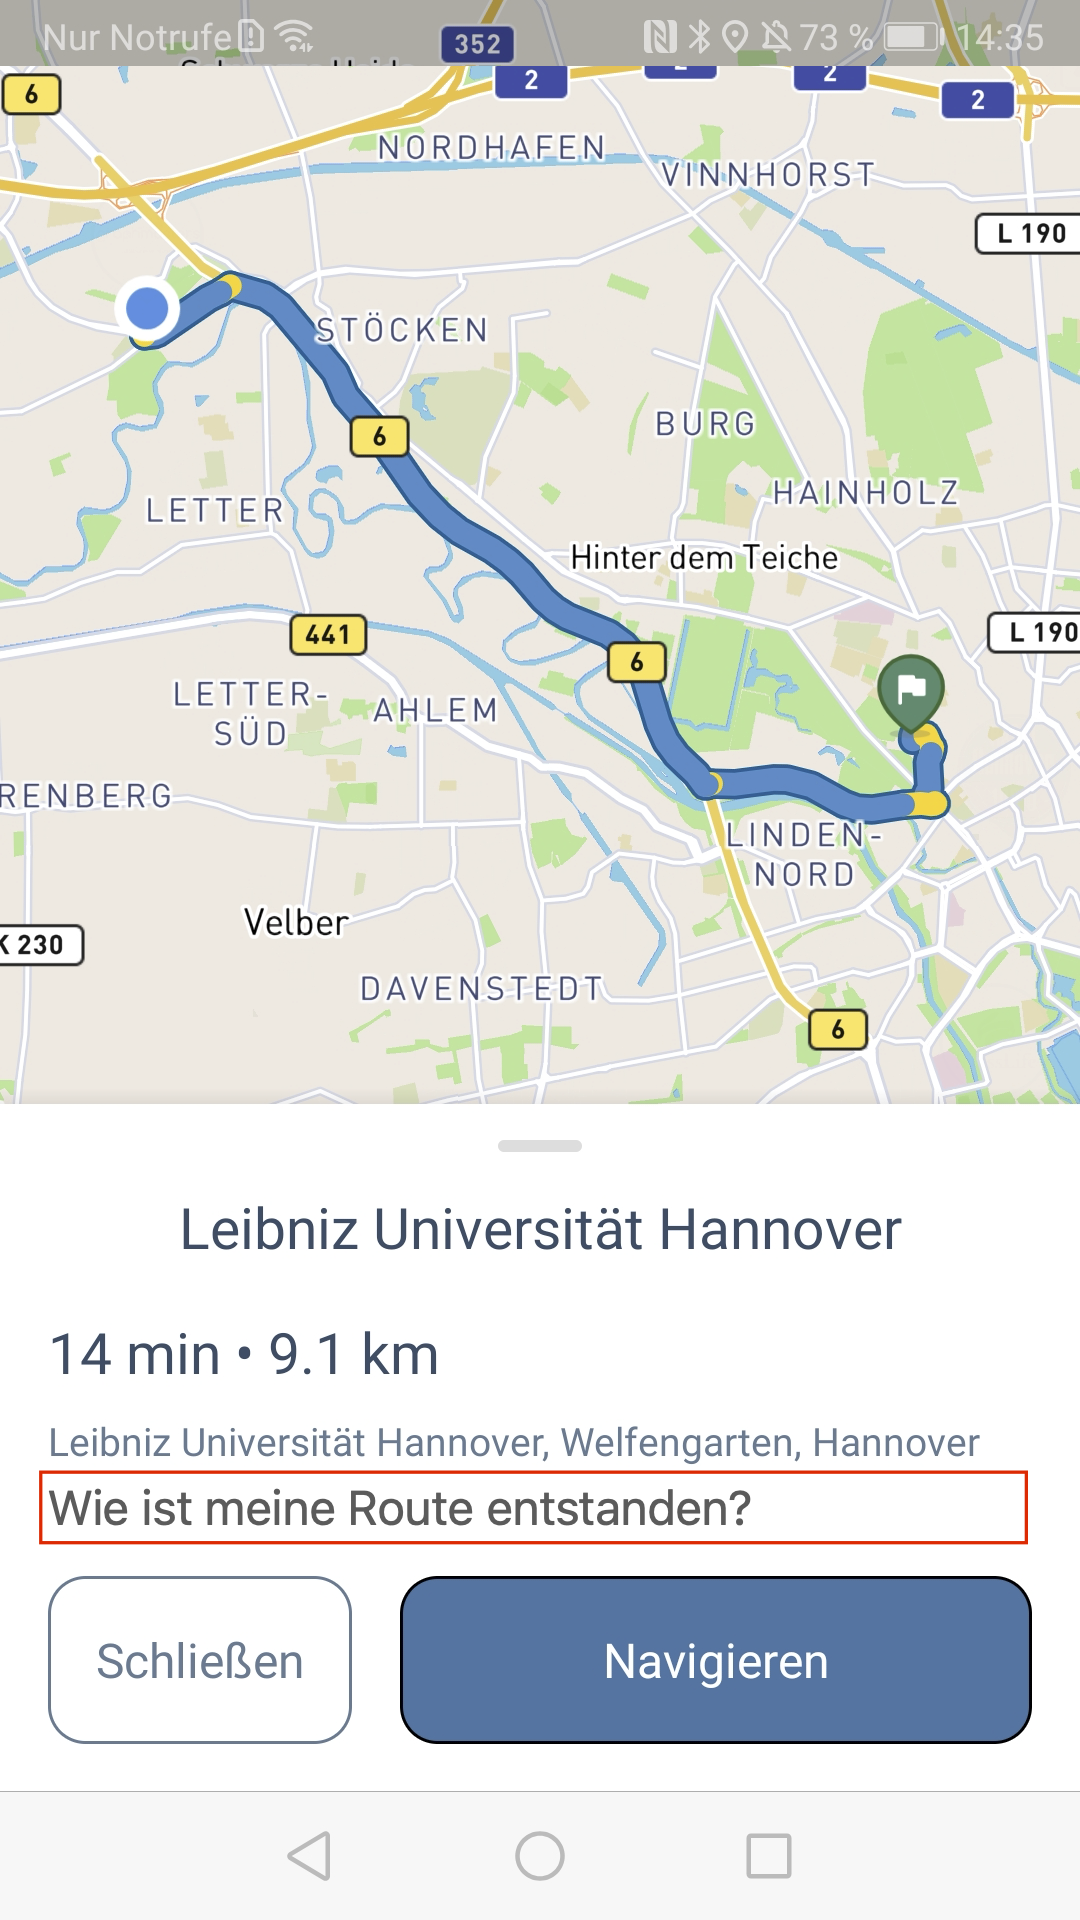
\includegraphics[width=.27\textwidth]{contents/06_model_evaluation/01_integration/res/02_routing_algorithm/prototype_1.png}
    }
    \hspace{.055\textwidth}
    \subfloat[Alternativer Prototyp zur Positionierung des Aufrufs der Erklärung]
    {
        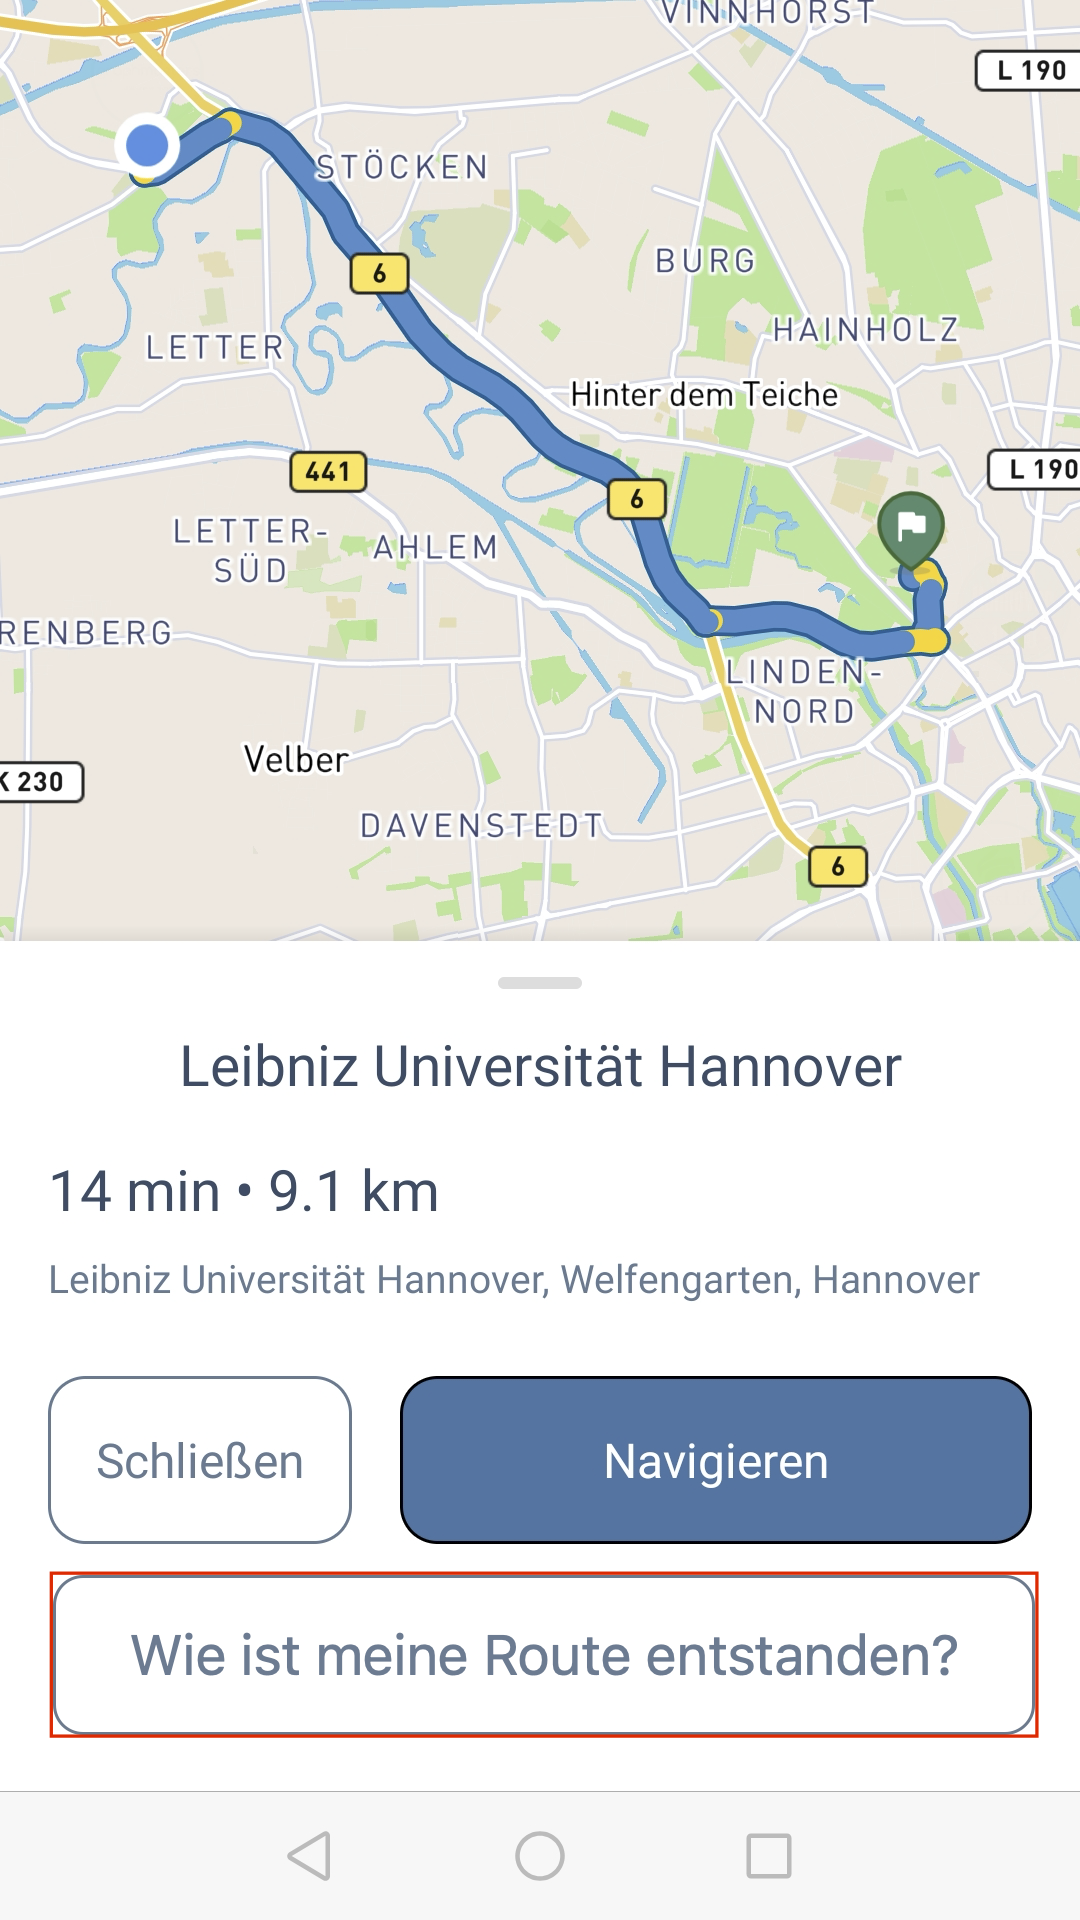
\includegraphics[width=.27\textwidth]{contents/06_model_evaluation/01_integration/res/02_routing_algorithm/prototype_2.png}
    }
    \hspace{.055\textwidth}
    \subfloat[Finales Design zur Positionierung des Aufrufs der Erklärung]
    {
        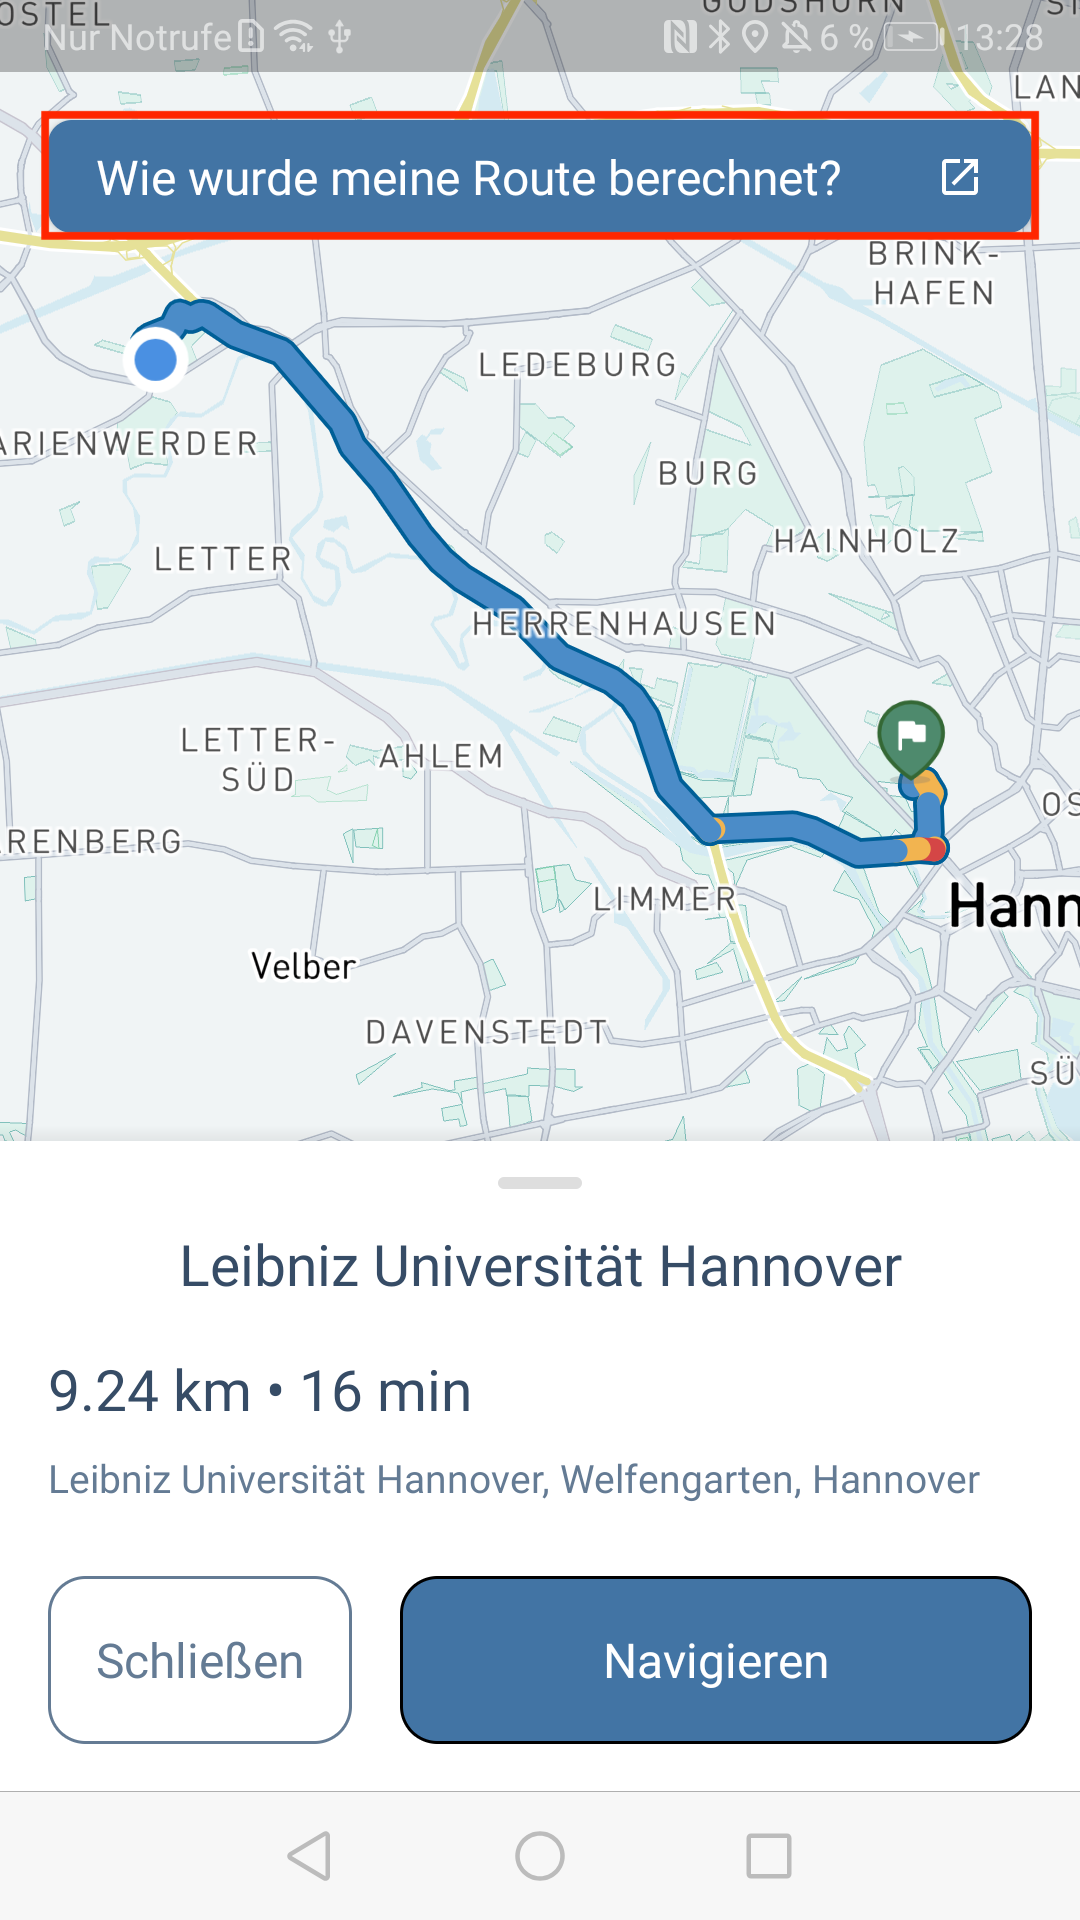
\includegraphics[width=.27\textwidth]{contents/06_model_evaluation/01_integration/res/02_routing_algorithm/final_1.png}
    }
    \caption{Prototyp und finale Designs für den Aufruf der Erklärung zu Einflüssen auf die Routenberechnung}
    \label{fig:prototype_routing_explanation}
\end{figure}

\subsubsection{Verkehrsaufkommen}
\label{sec:traffic_volume_definition}

\paragraph{[FR3]} \textit{NUNAV Navigation} muss den \textit{End Usern} während der Navigation Informationen zum Verkehrsgeschehen auf der aktuellen Route liefern.

Wie aus der Persona von Michael hervorgeht, wundert er sich zum Teil, warum \textit{NUNAV Navigation} aus seiner Sicht \glqq komische\grqq{} Routen vorschlägt. Ein Erklärungsansatz ist, das Verkehrsgeschehen auf der aktuellen Route anzuzeigen. Diese \textit{Context}-Information soll dabei helfen zu verstehen, warum \textit{NUNAV Navigation} andere Routen wählt. 

Dies ist allerdings nicht trivial, da die Berechnung des Verkehrsaufkommens und dessen subjektive Wahrnehmung der \textit{End User} nicht klar ist. Ein weiteres Problem ist, dass es nicht möglich ist, zu berechnen, welche Route für Nutzer auf der gleichen Strecke subjektiv als \glqq normal\grqq{} empfunden wird. Nachdem mehrere Lösungsansätze für dieses Problem in kleinen Runden bei \textit{Graphmasters} diskutiert wurden, wird als Lösung die Berechnung des Verhältnisses von durchschnittlicher Dauer der Route zu aktueller Dauer als Basiswert genommen. Die Daten werden dabei durch \textit{Nugraph} zur Verfügung gestellt und im Rahmen dieser Arbeit im \textit{BFF} auf die Stufen \glqq wenig Verkehr\grqq{}, \glqq mäßiger Verkehr\grqq{} und \glqq viel Verkehr\grqq{} abgebildet. Außerdem gibt es eine \glqq normale\grqq{} Verkehrssituation, in der den \textit{End Usern} keine Erklärung angezeigt wird. Die Abbildungsfunktion ist in den Zusatzmaterialien zu finden. Die Schwellwerte wurden intern durch Testfahrten ermittelt.

Die Informationen können \textit{End User} auf drei Wegen erhalten. Zunächst werden die Informationen in der Routenvorschau angezeigt. Dabei wird die Gesamtfahrzeit für die Route je nach Verkehrsaufkommen grün (wenig Verkehr), Standardtextfarbe (normaler Verkehr), orange (mäßiger Verkehr) und rot (viel Verkehr) dargestellt. Da im ersten Prototypen aufgefallen ist, dass die Farben alleine nicht aussagekräftig sind (siehe \autoref{fig:prototype_traffic_volume_route}, (a)), wurde zusätzlich ein kurzer Erklärungstext eingefügt (siehe \autoref{fig:prototype_traffic_volume_route}, (b)). Dieser ist bei \glqq normalem\grqq{} nicht zu sehen. So lernen die \textit{End User} mit der Zeit die Bedeutung der Farben. Eine Übersicht mit allen Prototypen ist in \autoref{sec:appendix_traffic_volume} zu finden.

Außerdem werden während der gesamten Navigation die Ankunftszeit und die Fahrzeit in der entsprechenden Farbe angezeigt und bei sich ändernder Verkehrssituation auch aktualisiert.

\begin{figure}[htb!]
    \centering
    \subfloat[Prototyp zur Darstellung des aktuellen Verkehrsaufkommens in der Routenvorschau]
    {
        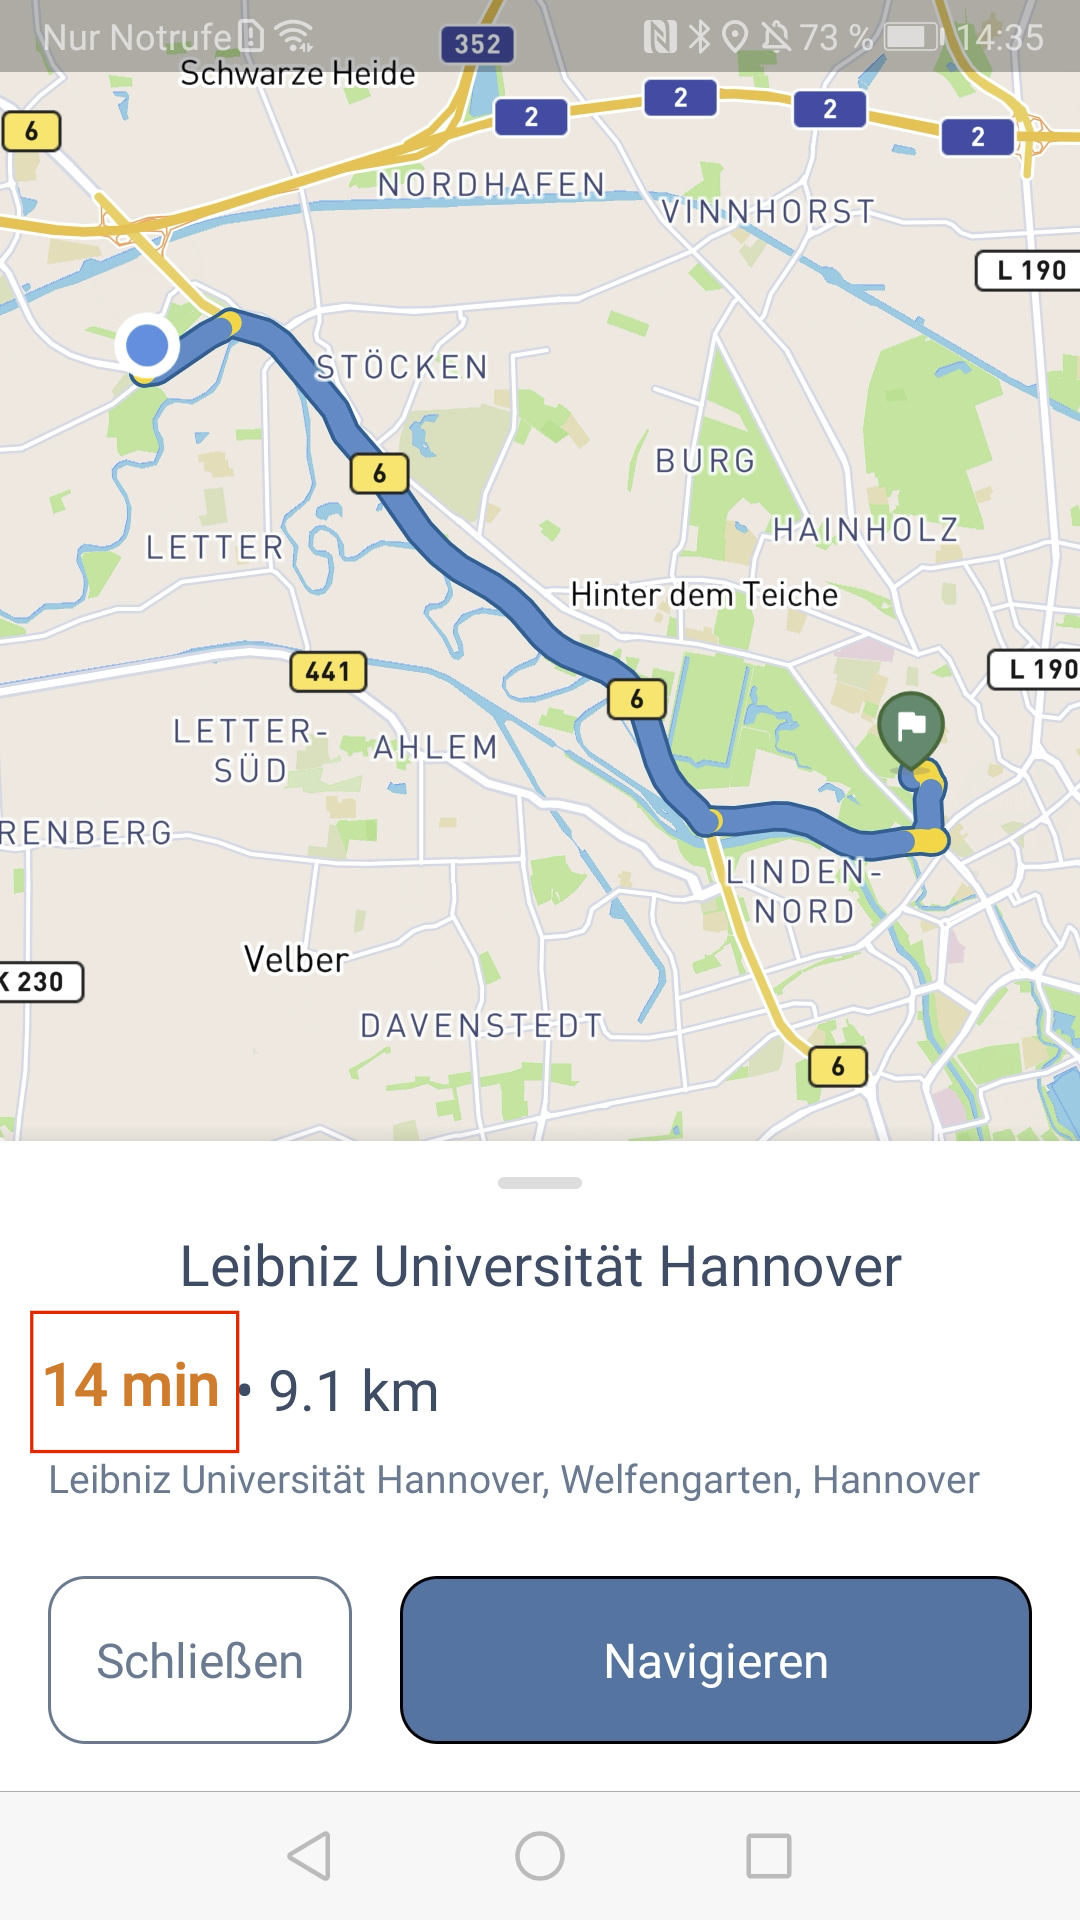
\includegraphics[width=.27\textwidth]{contents/06_model_evaluation/01_integration/res/03_traffic_volume/prototype_11.png}
    }
    \hspace{.055\textwidth}
    \subfloat[Finales Design zur Darstellung des aktuellen Verkehrsaufkommens in der Routenvorschau]
    {
        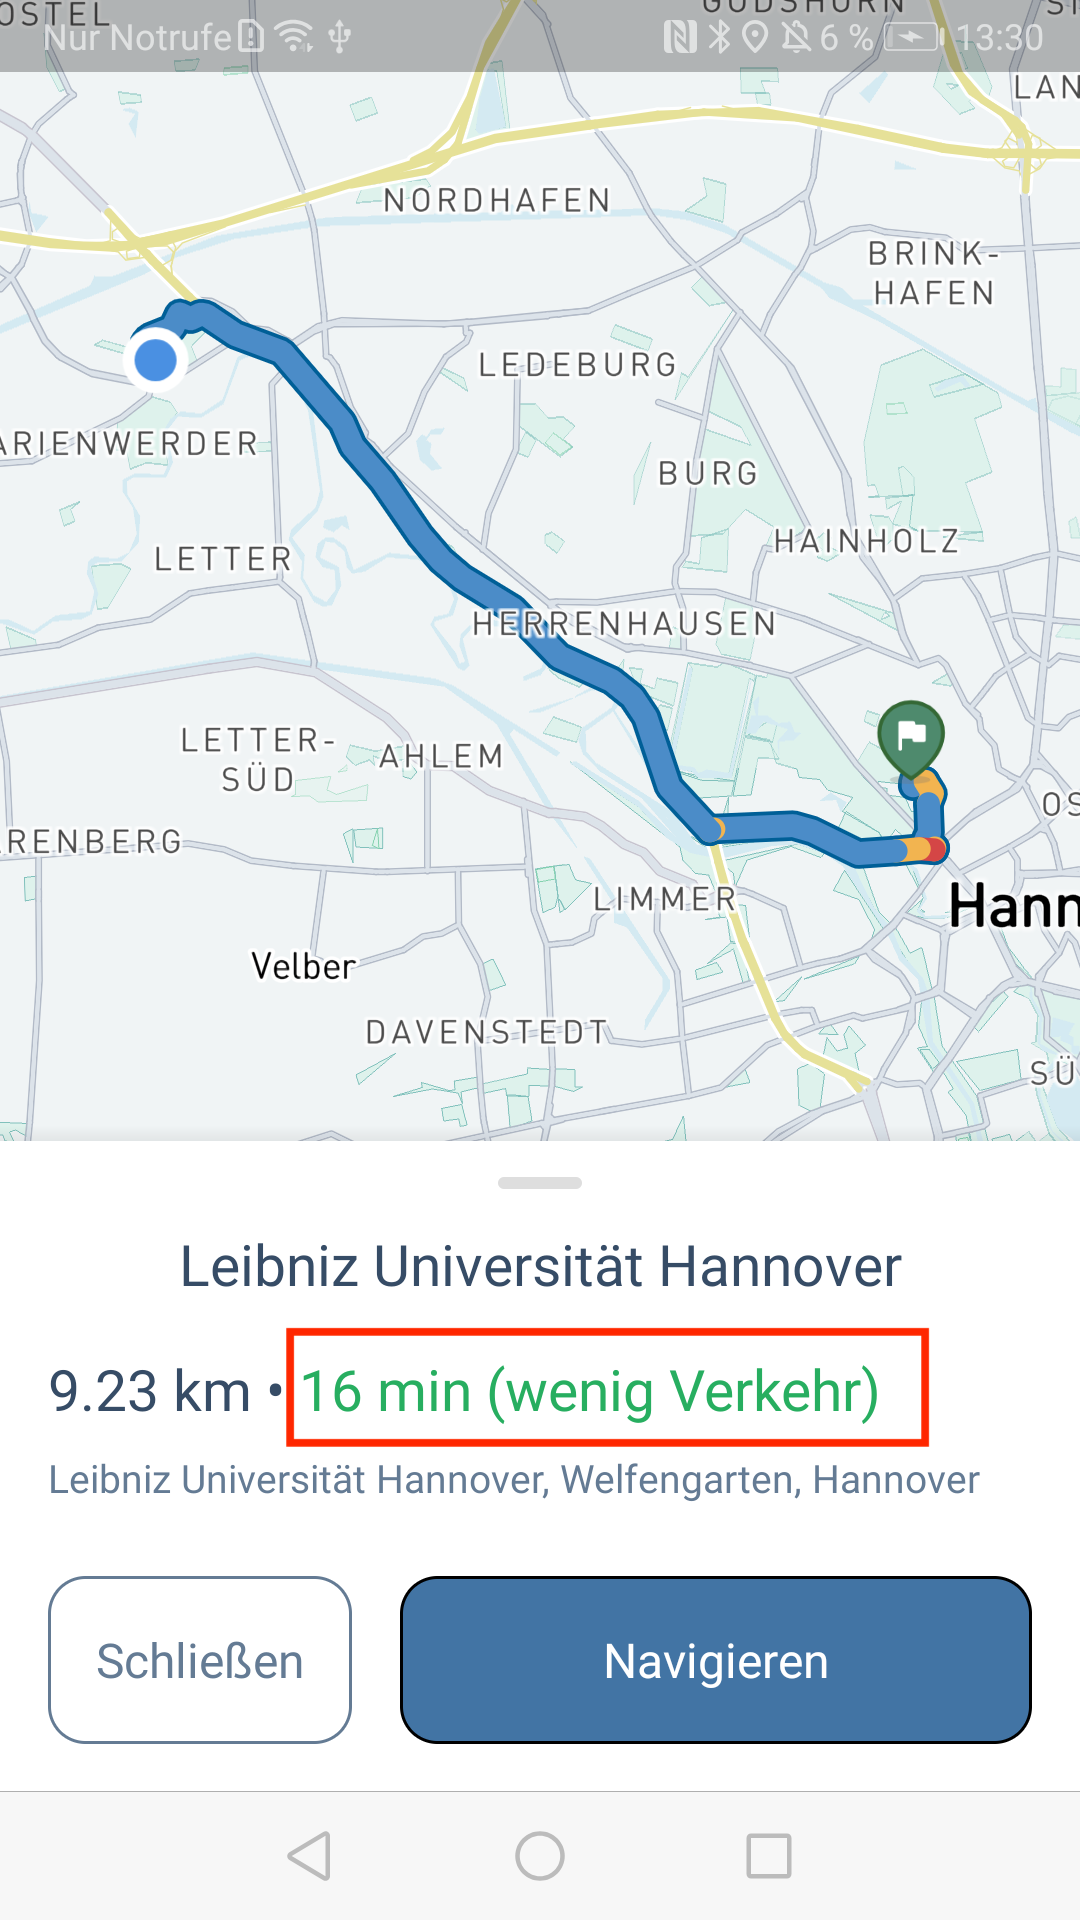
\includegraphics[width=.27\textwidth]{contents/06_model_evaluation/01_integration/res/03_traffic_volume/final_10.png}
    }
    \hspace{.055\textwidth}
    \subfloat[Finales Design zur Darstellung des aktuellen Verkehrsaufkommens während der Navigation]
    {
        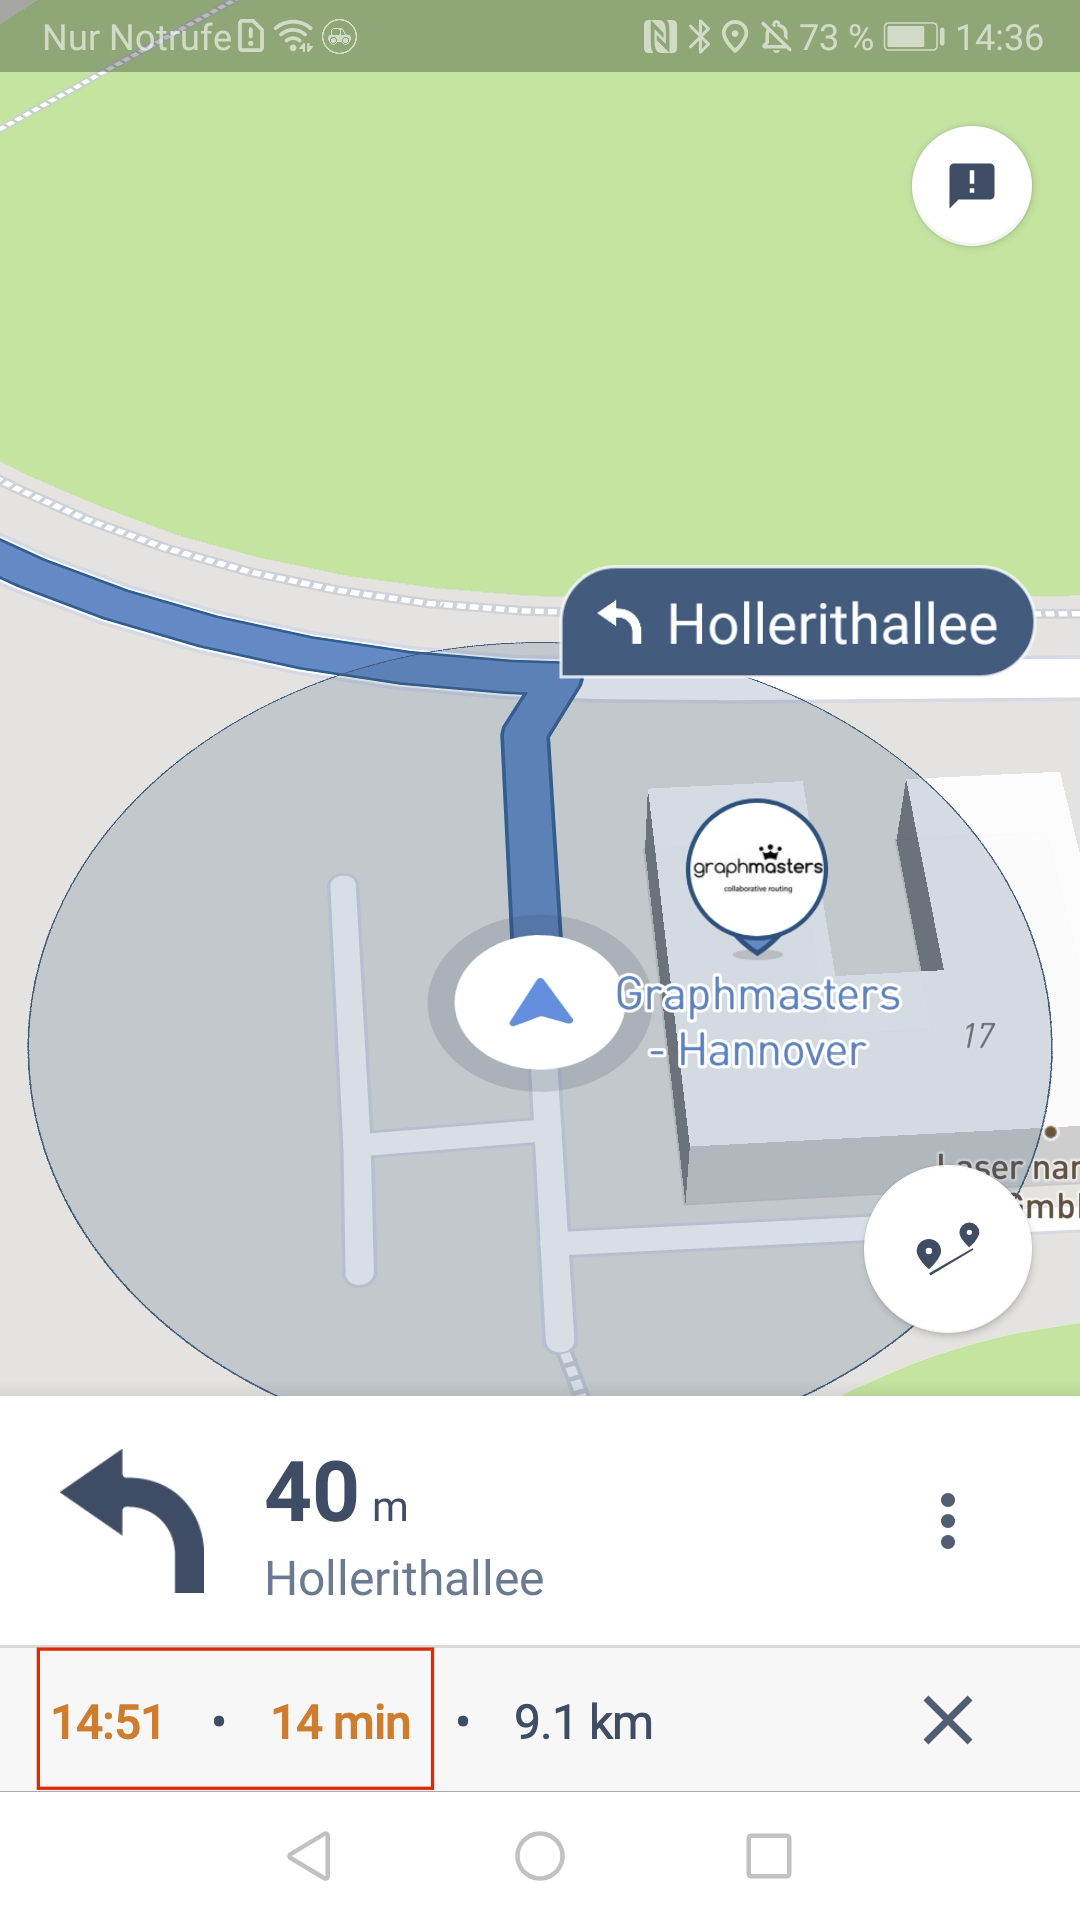
\includegraphics[width=.27\textwidth]{contents/06_model_evaluation/01_integration/res/03_traffic_volume/final_20.png}
    }
    \caption{Prototyp und finale Designs für die Erklärung zum kollaborativem Routing}
    \label{fig:prototype_traffic_volume_route}
\end{figure}

Des Weiteren ist das Sprachkommando, welches bei Start der Navigation gegeben wird, je nach Verkehrssituation unterschiedlich (siehe \autoref{tab:voice_commands_traffic_volume}).

\begin{table}[bht!]
    \begin{tabular}{p{.25\textwidth}p{.71\textwidth}}
        \hline
        Verkehrsaufkommen        & Sprachkommando \\
        \toprule
        wenig & Heute sind die Straßen frei. Du wirst dein Ziel <Zielname> um <Uhrzeit> erreichen. \\
        \tablerowspacing
        normal & Du wirst dein Ziel <Zielname> um <Uhrzeit> erreichen. \\
        \tablerowspacing
        mäßig & Da heute etwas mehr los ist, wirst du dein Ziel <Zielname> um <Uhrzeit> erreichen. \\
        \tablerowspacing
        viel & Da heute sehr viel los ist, wirst du dein Ziel <Zielname> um <Uhrzeit> erreichen. \\
        \toprule
    \end{tabular}
\caption{Sprachkommandos zum Start der Navigation abhängig von der Verkehrssituation}
\label{tab:voice_commands_traffic_volume}
\end{table}

\subsubsection{GPS-Qualität}
\label{sec:gps_accuracy_definition}

\paragraph{[FR4]} Wenn die Genauigkeit der Positionierung unzuverlässig ist, muss \textit{NUNAV Navigation} den \textit{End Usern} anzeigen, dass die Positionierung aktuell nicht zuverlässig ist.

Die letzte entwickelte Erklärung betrifft den Aspekt der \textit{Scrutability}. Ziel ist es \textit{End Usern} anzuzeigen, wenn sie sich aktuell auf die Position auf der Route nicht verlassen können. Dies ist zum Beispiel in Tunneln der Fall und besonders kritisch, wenn in Kürze ein Abbiege-Kommando erfolgt und somit an der falschen Stelle kommt. Bewusst wurde auf die technische Bezeichnung \glqq GPS\grqq{} verzichtet.

\begin{figure}[htb!]
    \centering
    \subfloat[Prototyp zum Design bei schlechtem GPS]
    {
        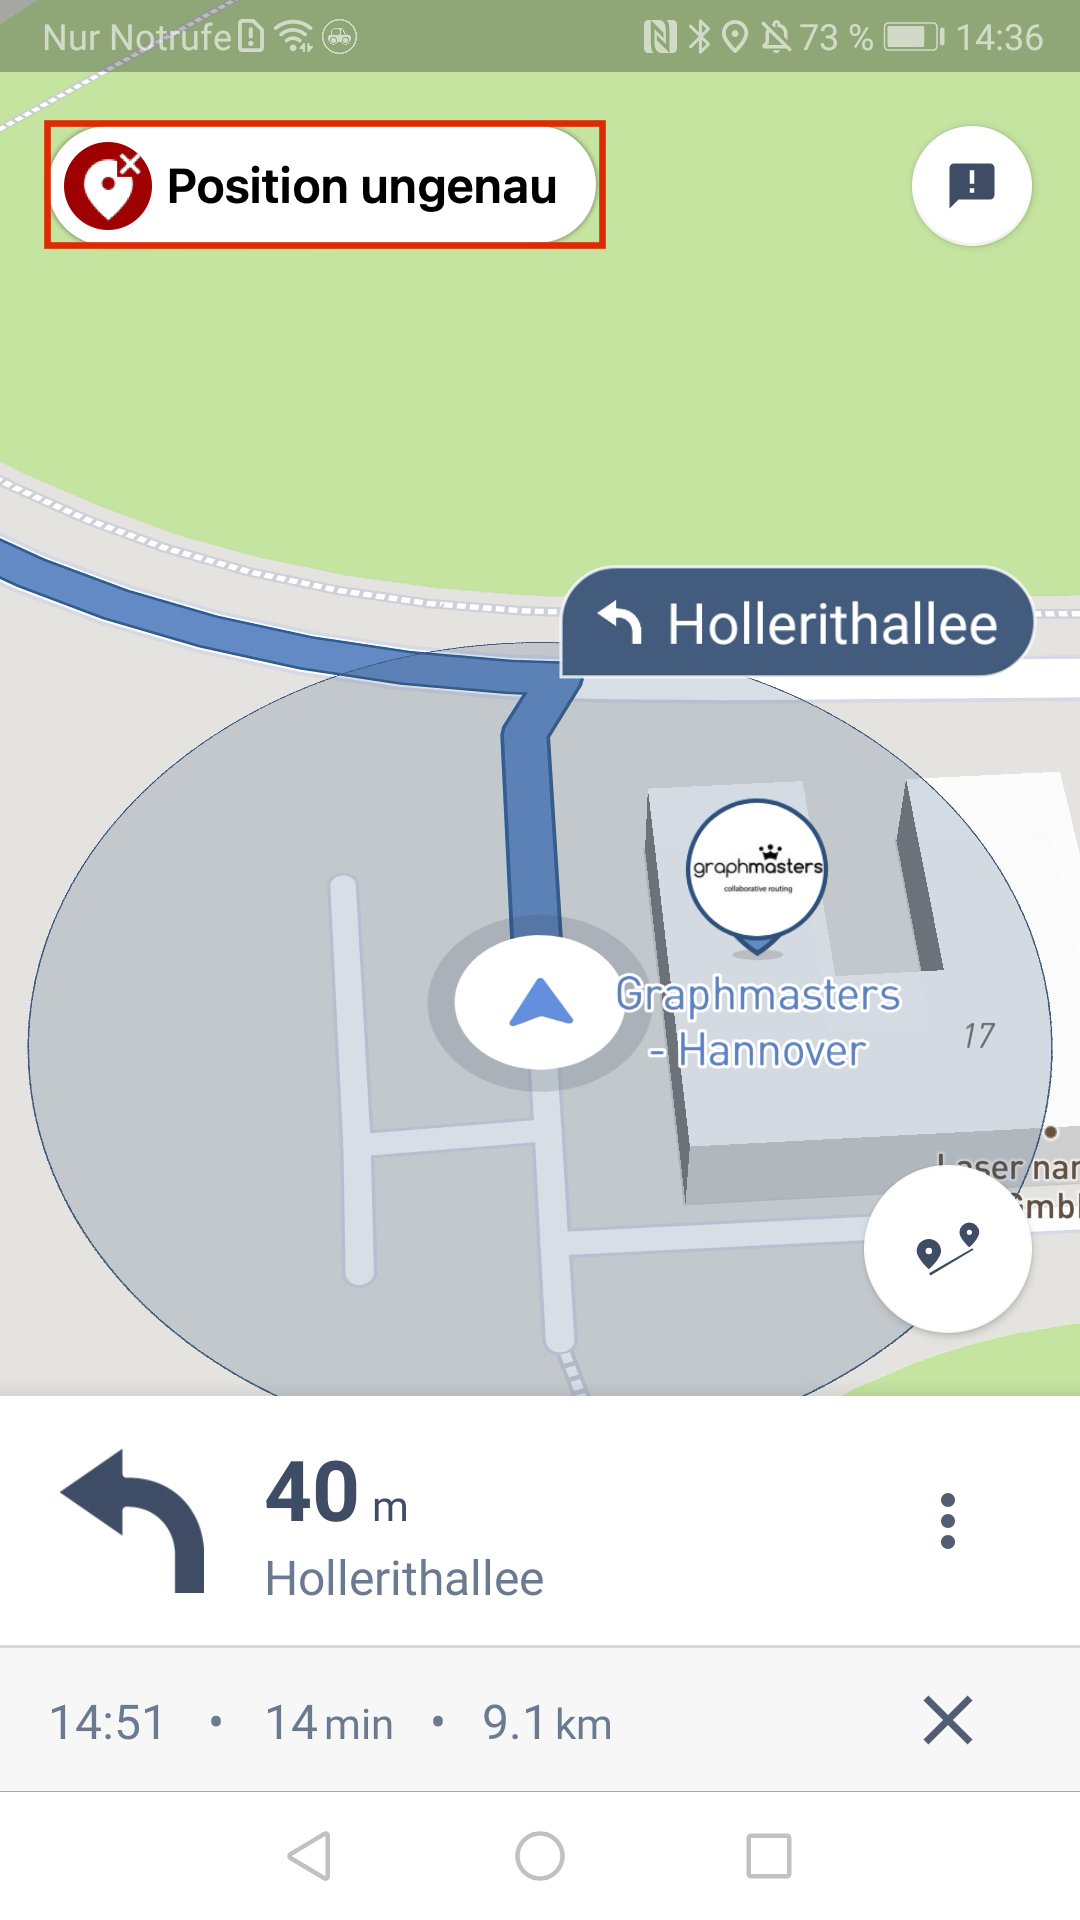
\includegraphics[width=.27\textwidth]{contents/06_model_evaluation/01_integration/res/04_position_accuracy/prototype_1.png}
    }
    \hspace{.055\textwidth}
    \subfloat[Finales Design bei schlechtem GPS]
    {
        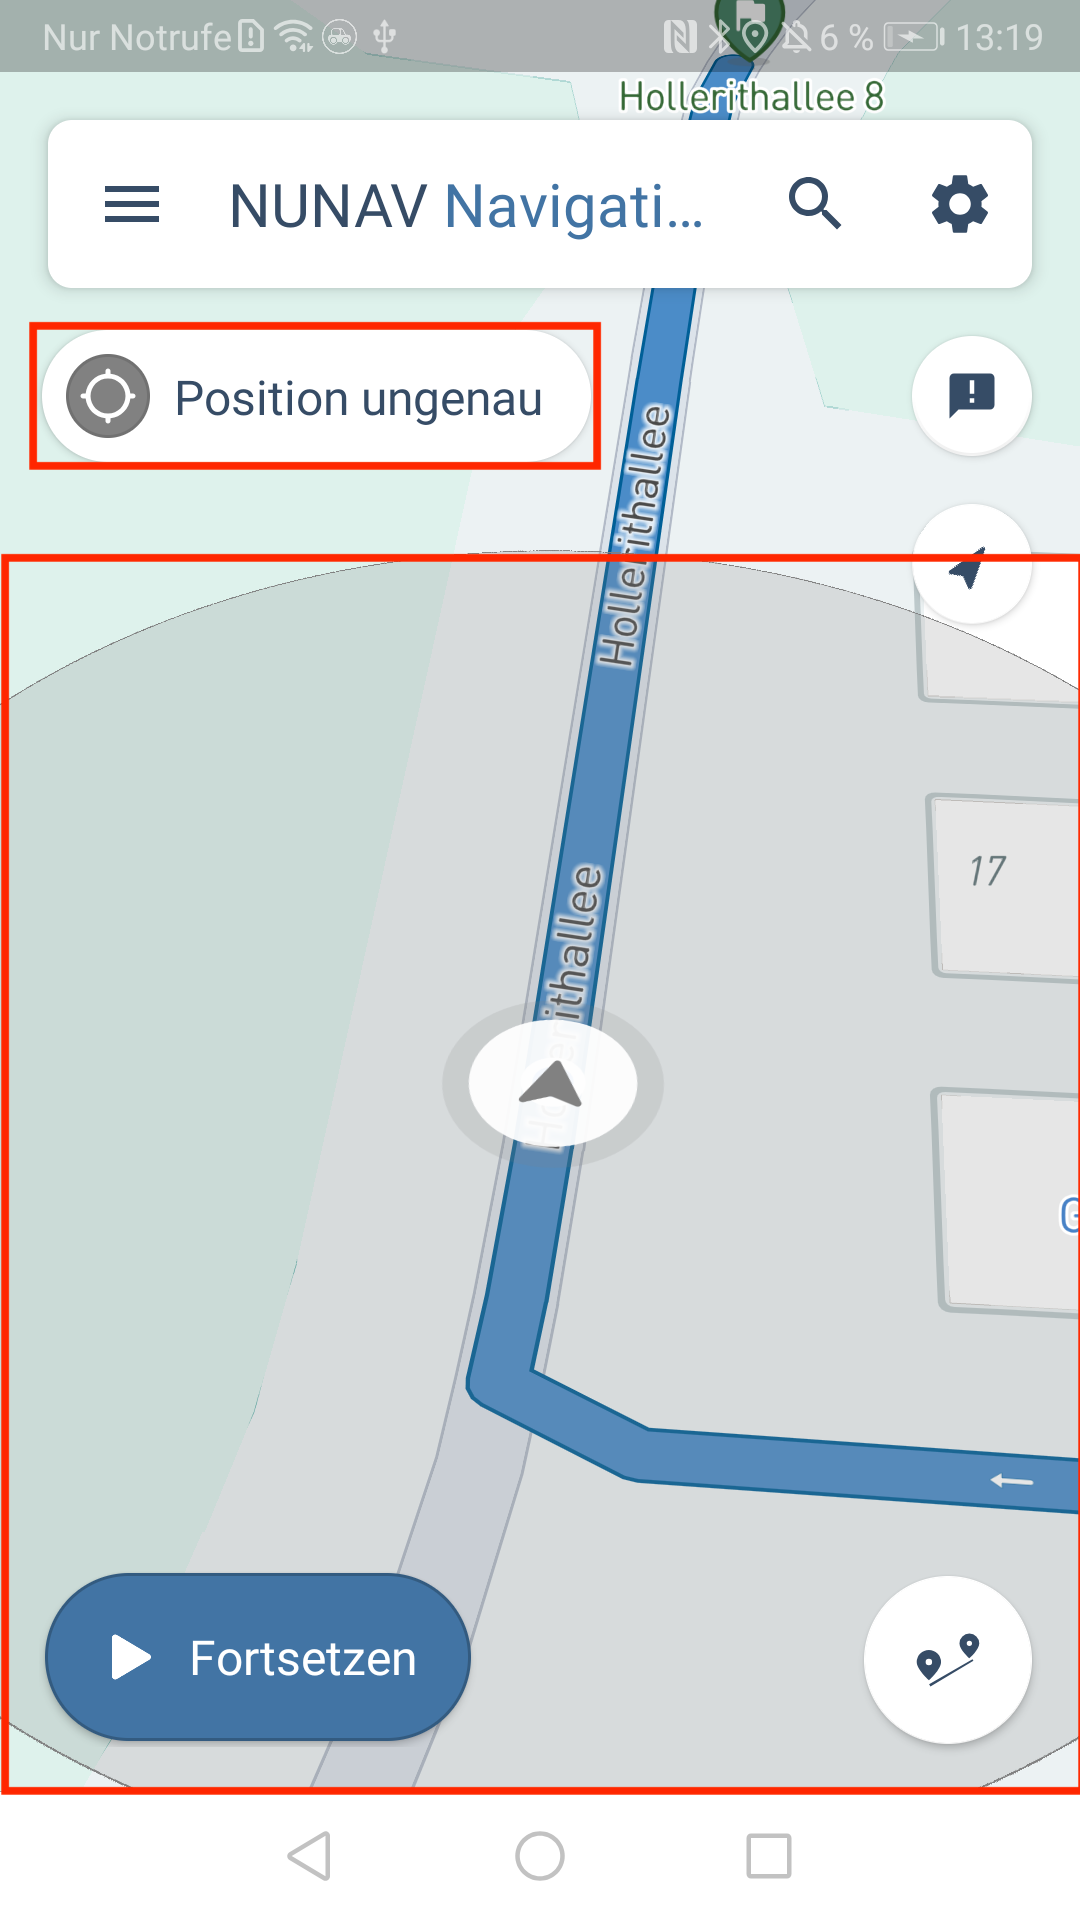
\includegraphics[width=.27\textwidth]{contents/06_model_evaluation/01_integration/res/04_position_accuracy/final_1.png}
    }
    \caption{Prototyp und finales Design für die Anzeige von schlechtem GPS während der Navigation}
    \label{fig:prototype_position_accuracy}
\end{figure}

Für die Entscheidung, wann das GPS ungenau ist, wurde innerhalb der \textit{NUNAV Navigation}-App ein neuer Algorithmus integriert, der diese trifft. Dabei spielt nicht nur die Genauigkeit, welche durch das GPS-Modul des Gerätes ermittelt wird, eine Rolle, sondern auch die Zeit, wann das letzte GPS-Update kam, da bei sehr schlechtem GPS keine Positionsupdates mehr vom Gerät geliefert werden. Der Algorithmus ist in den Zusatzmaterialien zu finden.

Als Design wurde im ersten Entwurf lediglich ein \textit{Growl} angezeigt und die Sprachansage \glqq Position ungenau\grqq{} ausgegeben. Insbesondere, wenn zum gleichen Zeitpunkt weitere \textit{Growls} angezeigt werden und die Sprachansagen vom \textit{End User} generell deaktiviert sind, hat sich die Sichtbarkeit bei Testfahrten als ungenügend herausgestellt. Daher wurde im finalen Entwurf zusätzlich das Positions-Icon auf der Karte und der Kreis, welcher die Genauigkeit der Position anzeigt, ausgegraut (siehe \autoref{fig:prototype_position_accuracy}, (b)).

\subsection{Umsetzung}



\section{Evaluation der Erklärungen}

\subsection{Ziel der Evaluation}

Das Ziel der Evaluation ist wie auch das Ziel der gesamten Arbeit (siehe \autoref{sec:goal_definition}) auf Basis der Vorlage von \citeauthor{wohlin2012experimentation} formuliert \cite{wohlin2012experimentation}.

\smallskip

\noindent\fbox{
    \parbox{0.964\textwidth}{
        \smallskip
        Die Studie \textbf{analysiert} die integrierten Erklärungen \textbf{in Bezug auf} die externe Qualität des Systems \textbf{zur} Evaluation \textbf{aus der Sicht} von \textit{End Usern} \textbf{im Kontext} der Benutzung von \textit{NUNAV Navigation}.
        \smallskip
    }
}

\smallskip

Dem zu Folge sollte im Rahmen der Evaluation überprüft werden, ob die zuvor aus den abgeleiteten Zielen von \textit{Graphmasters} definierten Qualitätsanforderungen durch die entwickelten Erklärungen erfüllt werden können.

\subsubsection{Hypothesen}
\label{sec:evaluation_hypothesis}

Die Überprüfung der Erfüllung der gestellten Qualitätsanforderungen erfolgt im Rahmen von Hypothesentests \cite{wohlin2012experimentation}. Grundsätzlich wurden zwei abstrakte Einflusshypothesen für die Integration der Erklärungen aufgestellt:

\begin{itemize}
    \item WENN die Studienteilnehmer Erklärungen erhalten, DANN ist ein positiver Einfluss auf die externe Softwarequalität messbar im Vergleich zu Teilnehmern, welche keine Erklärungen erhalten.
    \item WENN die Studienteilnehmer mehrere Erklärungen erhalten, DANN ist ein positiver Einfluss auf die externe Softwarequalität messbar im Vergleich zu Teilnehmern, welche nur eine Erklärung erhalten.
\end{itemize}

\subsection{Studienaufbau}

Ein Ergebnis des durchgeführten Workshops war, dass die Erklärungen nach Möglichkeit unter Realbedingungen evaluiert werden sollen. Daraus ist die Anforderung abgeleitet worden, dass eine Studie die \textit{End User} von \textit{NUNAV Navigation} so wenig wie möglich bemerken sollten. Daher kommen lediglich Verhaltensmetriken oder bereits in der Anwendung integrierte Metriken zum Einsatz.

Die genutzten Metriken wurden aus dem \autoref{sec:explanation_requirements} zur Definition der Anforderungen übernommen und sind bereits vor Beginn dieser Arbeit in \textit{NUNAV Navigation} integriert gewesen.

Aufgrund von Einflusshypothesen durch Störgrößen wurden neben den Erklärungsmetriken zusätzliche Metriken in die Anwendung integriert. Das Ziel dabei war es, auf der Basis möglicher Einflüsse Datensätze herausfiltern zu können, welche die Ergebnisse der Analyse der Einflüsse durch integrierte Erklärungen zu verzerren (siehe \autoref{sec:evaluation_other_dependencies}).

\subsection{Studiendurchführung}

Insgesamt wurde folglich eine zwei-wöchige Case Study als empirische Strategie gewählt. Um die Unterschiede in Bezug auf die externe Qualität messen zu können, wurden nicht allen Teilnehmern die Erklärungen angezeigt. Zusätzlich sollte nicht nur eine Veränderung durch die Erklärungen messbar gemacht werden, sondern auch zwischen den einzelnen entwickelten Erklärungen unterschieden werden. Trotz dessen sollte auch die Kombination der verschiedenen Erklärungen überprüft werden. Um jedoch für jede Bedingung genug Nutzer als Datengrundlage zu haben, wurden nicht alle verschiedenen Kombinationsmöglichkeiten der Erklärungen überprüft.

Grundsätzlich wurden die Erklärungen in die zwei Gruppen \textit{statische} und \textit{Context}-abhängige Erklärungen gegliedert. Unter den statischen Erklärungen sind die beiden Erklärungen, welche den Routingalgorithmus und die Einflüsse auf die Routenberechnung erklären, zusammengefasst (siehe \autoref{sec:explanation_design}).

Analog dazu sind die \textit{Context}-Erklärungen zum aktuellen Verkehrsaufkommen und zu Positionsungenauigkeiten während der Navigation als eine Bedingung für die Studie zusammengefasst worden (siehe \autoref{sec:traffic_volume_definition} und \autoref{sec:gps_accuracy_definition}).

Insgesamt sind folglich vier verschiedene Studiengruppen entstanden:

\begin{itemize}
    \item \textbf{Gruppe 1}: Nutzer, die keine Erklärungen erhalten
    \item \textbf{Gruppe 2}: Nutzer, die statische Erklärungen erhalten
    \item \textbf{Gruppe 3}: Nutzer, die \textit{Context}-abhängige Erklärungen erhalten
    \item \textbf{Gruppe 4}: Nutzer, die statische als auch \textit{Context}-abhängige Erklärungen erhalten
\end{itemize}

Für die Zuordnung der einzelnen Studiengruppen wurde das im Rahmen dieser Arbeit entwickelte \textit{Feature-Flag}-System verwendet. Anhand von zufällig generierten Identifikatoren wurde zu diesem Zweck ein Hashwert berechnet und die Teilnehmer anhand der Teilbarkeit durch vier, den einzelnen Gruppen zugeordnet (siehe Zusatzmaterialien).

\newpage

\subsection{Studienablauf}

\subsection{Ergebnisse}
\label{sec:study_results_quantitativ}

\subsubsection{Übersicht}

% \begin{table}[htb!]
%     \begin{center}
%         \begin{tabular}{p{.3\textwidth} p{.3\textwidth} p{.3\textwidth}}
%             \hline
%             Daten & Datentyp & Anzahl \\
%             \toprule
%             Teilnehmer          & insgesamt & 9 745 \\
%                                 & gefiltert & 4 012 \\
%             \tablerowspacing
%             Gefahrene Routen    & insgesamt & 41 540 \\
%                                 & gefiltert & 16 531 \\
%             \toprule
%         \end{tabular}
%     \end{center}
%     \caption{Evaluation}
%     \label{tab:study_user_overview}
% \end{table}

Um bei der Analyse der Daten, Nutzer auszuschließen, die eine Navigation nur gestartet haben, um sich diese anzusehen, aber NUNAV nicht aktiv während einer Autofahrt genutzt haben werden Routen, die kürzer als 5 Kilometer sind herausgefiltert. 
%Dies verhindert außerdem, dass das Gelangen zur ersten Route, sowie das Suchen von Parkplätzen einen zu großen Einfluss auf die Daten haben

Für Nutzer der Gruppen 3 und 4 kann es passieren, dass sie keine Erklärung während der Navigation erhalten, wenn die aktuelle Route keiner Erklärung bedarf. Dies ist der Fall, wenn das Verkehrsaufkommen \glqq normal\grqq{} ist und der Nutzer während der gesamten Fahrt guten GPS-Empfang hat (Definitionen siehe \autoref{sec:gps_accuracy_definition}). Bei der Betrachtung von einzelnen Routen werden die Teilnehmer folglich in die Gruppen 1 oder 2 umsortiert, falls sie während der Navigation keine Erklärung gesehen haben. Wird eine Metrik analysiert, die sich pro Nutzer über mehrere Routen erstreckt, werden die Teilnehmer den Gruppen zugeordnet, wenn NUNAV ihnen mindestens einmal eine Erklärung aus der Studiengruppe angezeigt hat. Über Übersicht findet sich in \autoref{tab:study_user_group_overview}

\begin{table}
    \centering
    \begin{tabular}{p{.26\textwidth} c c c}
        \hline
        \multirow{2}{*}{Studiengruppe} & \multirow{2}{*}{Anzahl der Nutzer} & \multicolumn{2}{c}{Anzahl der Routen} \\
        & & Insgesamt & Mit Nutzerbewertung \\
        \toprule
        Gruppe 1            & 1 778  & 4 807  & 133 \\
        Gruppe 2            & 1 397  & 3 413  & 135 \\
        Gruppe 3            & 468   & 4 571  & 184 \\
        Gruppe 4            & 369   & 3 740  & 173 \\
        \midrule
        \textbf{Insgesamt}  & 4 012  & 16 531 & 625 \\ 
        \toprule
    \end{tabular}
    \caption{Übersicht über die Daten der Studiengruppen}
    \label{tab:study_user_group_overview}
\end{table}

\subsubsection{Einflüsse außerhalb von Erklärungen}

Um auszuschließen, dass die untersuchten Variablen von weiteren Faktoren abhängen habe wurde zu Beginn geprüft, ob eine schlecht vorausgesagte Ankunftszeit oder mehrfach auftretendes schlechtes GPS einen Effekt auf die Anzahl der Abweichungen von der Route oder die Zufriedenheit mit der Route haben. Dies geschieht, da es Vermutungen eines negativen Zusammenhangs gab, der die Ergebnisse der Untersuchung der integrierten Erklärungen beeinflussen könnte. Dazu wurde die Kontrollgruppe (Gruppe 1: Ohne Erklärungen) untersucht.

Die 4 Hypothesen lauten wie folgt:

\begin{enumerate}
    \item[1.1] WENN die ATA mehr als 10 \% und mindestens 2 Minuten von der ETA abweicht, DANN hat dies einen signifikant messbaren negativen Einfluss auf die Nutzerzufriedenheit.
    \item[1.2] WENN die ATA mehr als 10 \% und mindestens 2 Minuten von der ETA abweicht, DANN ist die Anzahl der Routenabweichungen signifikant messbar höher.
    \item[1.3] WENN NUNAV auf der betrachteten Route pro 5 km durchschnittlich mindestens eine Positionsungenauigkeit aufwies, DANN hat dies einen signifikant messbaren negativen Einfluss auf die Nutzerzufriedenheit.
    \item[1.4] WENN NUNAV auf der betrachteten Route pro 5 km durchschnittlich mindestens eine Positionsungenauigkeit aufwies, DANN ist die Anzahl der Routen-Abweichungen signifikant messbar höher.
\end{enumerate}

Bei der statistischen Prüfung der Auswirkung von schlecht vorausgesagte Ankunftszeit auf die Anzahl der Routen-Abweichungen mittels eines Kruskal-Wallis-Tests lässt sich kein Haupteffekt feststellen ($ p = 0.197648 > 0.05 $). Gleiches gilt für die Überprüfung eines Effektes auf die Nutzerzufriedenheit ($ p = 0.564911 > 0.05 $). Folglich können die Hypothesen 1.1 und 1.2 abgelehnt werden.

Für die Überprüfung, ob eine schlechte Positionierung einen Effekt auf die Nutzerzufriedenheit hat, hat ein Kruskal-Wallis-Test ergeben, dass kein signifikanter Effekt vorliegt ($ p = 0.269231 > 0.05 $). Folglich kann Hypothese 1.3 abgelehnt werden. Bei der Prüfung von Hypothese 1.4 hat sich herausgestellt, dass die Anzahl der Routen-Abweichungen signifikant höher ist, wenn es im Durchschnitt mehr als ein mal pro 5 km eine Positionsungenauigkeit gibt ($ p = 3.426601e-15 < 0.05 $  $ \mu_{good gps}=efse $ $ \mu_{bad gps}=efse $). Folglich kann Hypothese 1.4 angenommen werden. Da eine häufige ungenaue Positionierung also bereits einen Einfluss auf die Anzahl der Abweichungen von der Route hat, werden Daten mit ungenauer Positionierung bei der Auswertung vom Einfluss von Erklärungen auf die Anzahl der Routen-Abweichungen nicht mitbetrachtet.

\subsubsection{Nutzerabweichungen von der vorgeschlagenen Route}

\textbf{Hypothesen}

\begin{enumerate}
    \item[2.1] WENN der Teilnehmer Erklärungen erhält, DANN folgt er signifikant häufiger der vorgeschlagenen Route als wenn er keine erhält.
    \item[2.2] WENN der Teilnehmer nur eine der beiden vorgestellten Erklärungstypen erhält, DANN folgt er signifikant weniger häufig der vorgeschlagenen Route als wenn ihm beide Arten von Erklärungen präsentiert werden.
\end{enumerate}

 Als Messwert wird die Anzahl der \textit{Offroutes} relativ zu Gesamtlänge der Route verwendet. Die Einheit ist Offroute pro Kilometer.

\smallskip

\noindent\colorbox{lightgray}{%
    \parbox{0.975\linewidth}{
        \textbf{Definition}

        Ein \textit{Offroute} ist der Fall, dass der Nutzer sich aktuell nicht auf der vorgeschlagenen Route befindet. Konkret bedeutet dies, dass das Smartphone NUNAV eine neue Position bereitstellt und nach einer Evaluation bestimmter Kriterien festgestellt wird, dass sich der Nutzer nicht mehr auf der Route befindet. In der Regel wird dann eine neue Route vom Server angefordert.
        
        \textit{Zu Beachten}
        \begin{itemize}
            \item Bis der Nutzer eine neue Route erhält, kann es mehrere \textit{Offroutes} geben.
            \item Es kann sein, dass der Nutzer mehrfach wieder die gleiche Route nach einem \textit{Offroute} erhält.
            \item Es kann auch zu einem \textit{Offroute} kommen, wenn die Nutzerposition schlecht ist.
        \end{itemize}
    }
}

\smallskip

Bei der Betrachtung von Abweichungen von der Route werden wie oben beschrieben Navigationen, bei denen es häufig zu einer ungenauen Positionierung kommt aus den Daten gefiltert. Außerdem wurde sie normalisiert, sodass schlussendlich 16 314 einzelne Navigationen zur Analyse der Routen-Abweichungen im Datensatz verblieben sind.

\begin{figure}
    \centering
    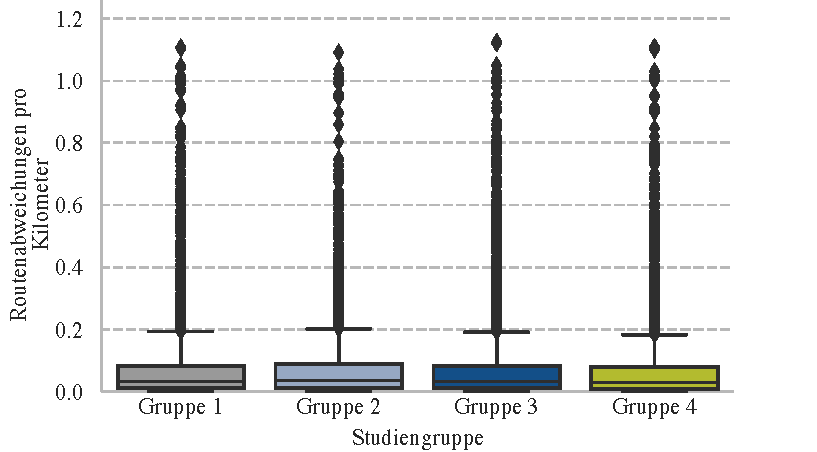
\includegraphics[width=\textwidth]{contents/06_model_evaluation/02_evaluation/res/off_route_result_overview.pdf}
    \caption{Anzahl der Offroutes pro Kilometer für jede Studiengruppe}
\end{figure}

\begin{table}
    \centering
    \begin{tabular}{|l|c|c|}
        \hline
        \textbf{Studiengruppe}  & \textbf{Mittelwert} [N/km] & \textbf{Standardabweichung} [N/km]\\ \hline
        Gruppe 1                & 0.0753 & 0.1293 \\ \hline
        Gruppe 2                & 0.0786 & 0.1272 \\ \hline
        Gruppe 3                & 0.0803 & 0.1410 \\ \hline
        Gruppe 4                & 0.0732 &  0.1328 \\ \hline
    \end{tabular}
    \caption{Übersicht der Ergebnisse der Routen-Abweichungen pro Kilometer}
    \label{tab:study_offroute_results}
\end{table}

Um zu prüfen, ob die Unterschiede der Mittelwerte signifikant sind, muss dies mittels eines statistischen Tests überprüft werden. Da es sich um ein Experiment von meheeren nicht zusammenhängenden Studiengruppen mit mehr als zwei verschiedenen Bedingungen handelt, kommen entweder ein ANOVA- oder Kruskal-Wallis-Test infrage. Für ersteren gilt, dass die Daten gleich verteilt sein müssen. Dies wurde mittels Shapiro-Wilk-Test geprüft. Da das Ergebnis für alle Test-Gruppen $ p = 0.0 < 0.05 $ ist, sind die Daten nicht normal verteilt. Folglich wird zur Signifikanzprüfung der Kruskal-Wallis-Test verwendet. Aufgrund des Ergebnisses von $ p = 0.000007 < 0.05 $, wird abgeleitet, dass ein Haupteffekt vorliegt.

Für die Prüfung zwischen welchen Studiengruppen ein signifikanter Unterschied vorliegt, wird der Dunn-Test \cite{dunn1964multiple} verwendet. (P wird mit der \glqq bonferoni\grqq{}-Methode korrigiert.)

Auch hier wird wieder von einem Signifikanzniveau $ p < 0.05 $ ausgegangen (siehe \nameref{ch:appendix_1}). Folglich weichen die Nutzer der Gruppe 4 signifikant weniger von der vorgeschlagenen Route ab als die Teilnehmer aller anderen Gruppen ($ p_{11} = 0.0288 $, $ p_{12} = 0.0000 $, $ p_{13} = 0.0030 $). Weitere signifikante Unterschiede gibt es nicht.

Hypothese 2.1 trifft zwar für das Geben aller Erklärungstypen (Gruppe 4) zu, nicht aber für die Gruppen 2 und 3. Folglich wird diese abgelehnt. Hypothese 2.2 kann angenommen werden, da die Nutzer der Gruppe 4 sowohl signifikant weniger von der vorgeschlagenen Route abgewichen sind als die Nutzer der Gruppe 2 sind als auch die Nutzer der Gruppe 3.

\subsubsection{Nutzerzufriedenheit mit der aktuellen Route}

Um die Zufriedenheit der Nutzer mit der abgeschlossenen Navigation zu evaluieren, setzt NUNAV auf eine Bewertung mithilfe von 5 Sternen bei Erreichen des Zieles. Dies ist verknüpft mit der Frage \glqq Wie hat dir die Fahrt gefallen\grqq (siehe \autoref{fig:screenshot_destination_reached}). Außerdem sind die Fahrtdauer und zurückgelegte Kilometer angegeben.

\begin{figure}
    \centering
    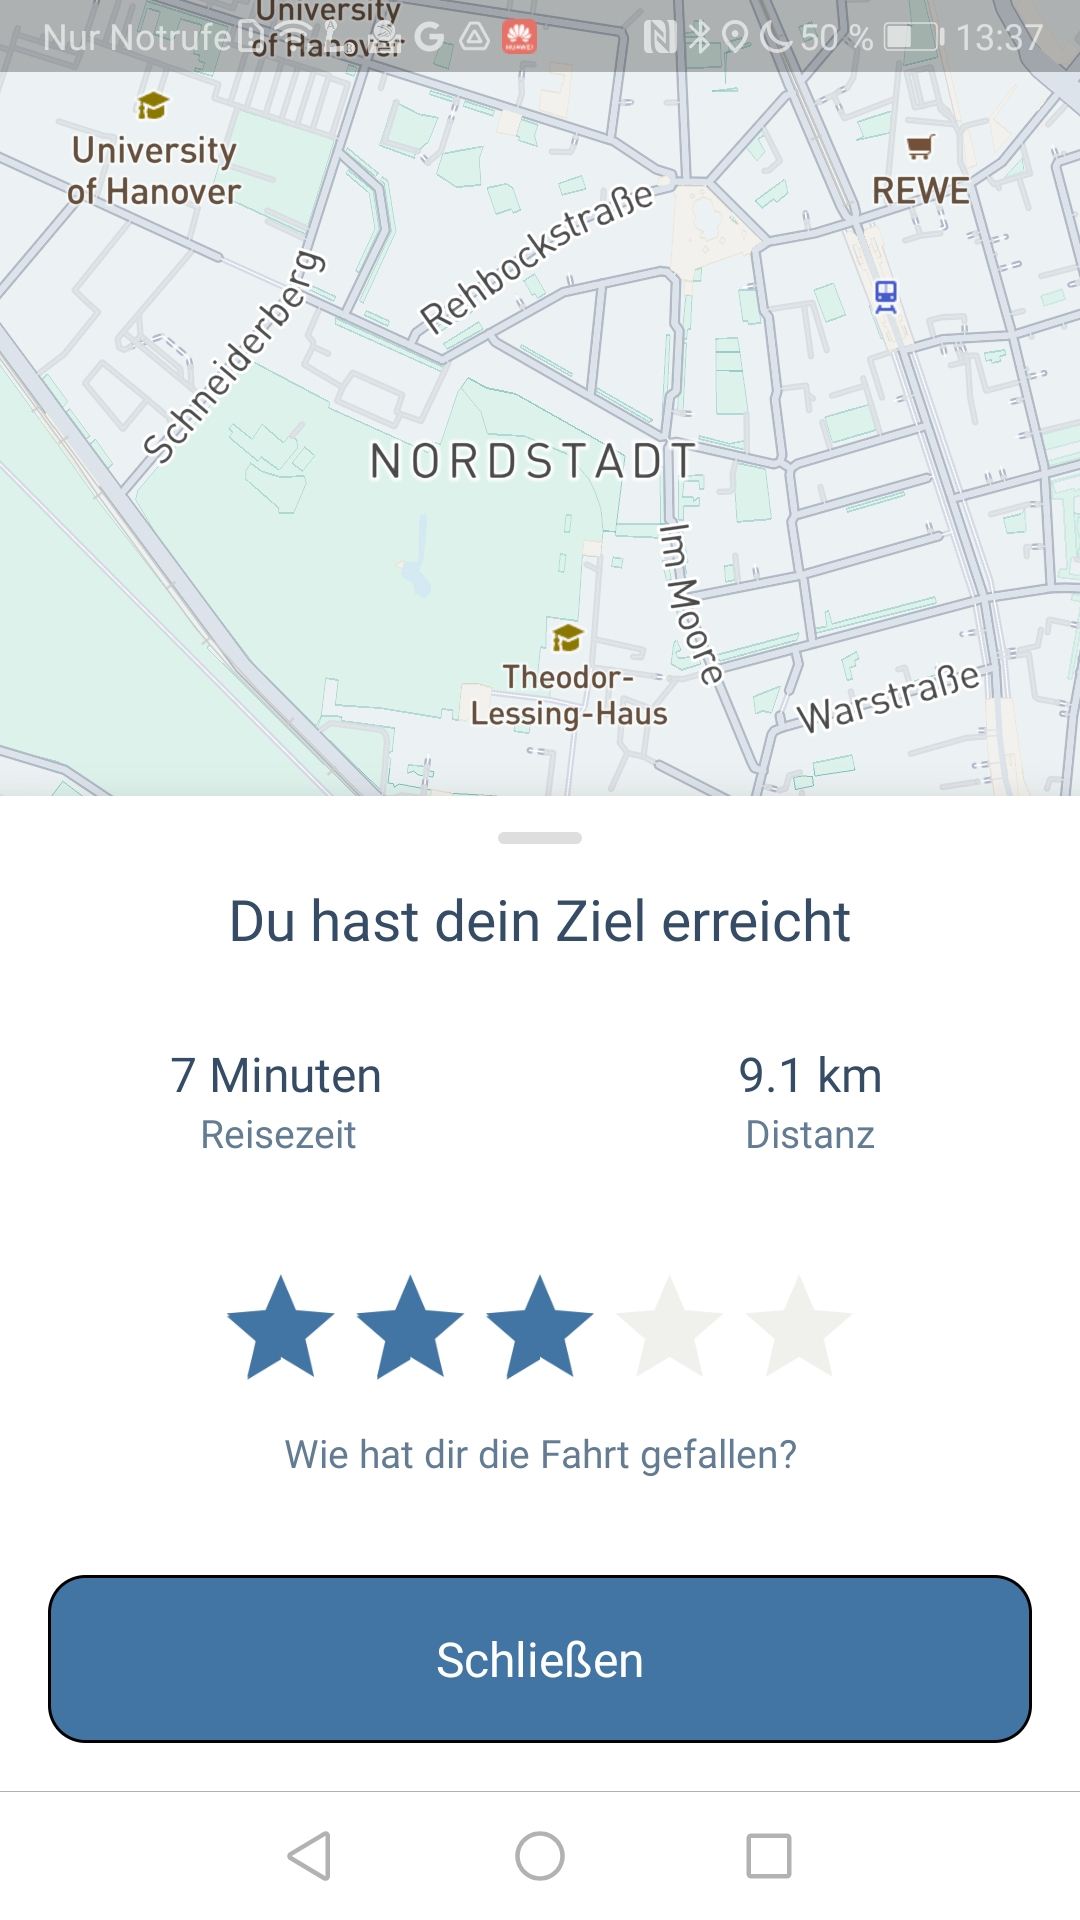
\includegraphics[width=0.27\linewidth]{contents/06_model_evaluation/02_evaluation/res/rating_screenshot.jpg}
    \caption{Bildschirmfoto des Bewertungsdialogs}
    \label{fig:screenshot_destination_reached}
\end{figure}

\textbf{Hypothesen}

\begin{enumerate}
    \item[3.1] WENN Teilnehmer Erklärungen erhalten, DANN geben sie im Vergleich eine signifikant höhere Bewertung für die Navigation ab, als wenn sie keine Erklärungen erhalten.
    \item[3.2] WENN Teilnehmer nur einen der beiden vorgestellten Erklärungstypen erhalten, DANN geben sie im Vergleich eine signifikant niedrigere Bewertung für die Navigation ab, als wenn sie beide Erklärungstypen erhalten.
\end{enumerate}

\begin{figure}
    \centering
    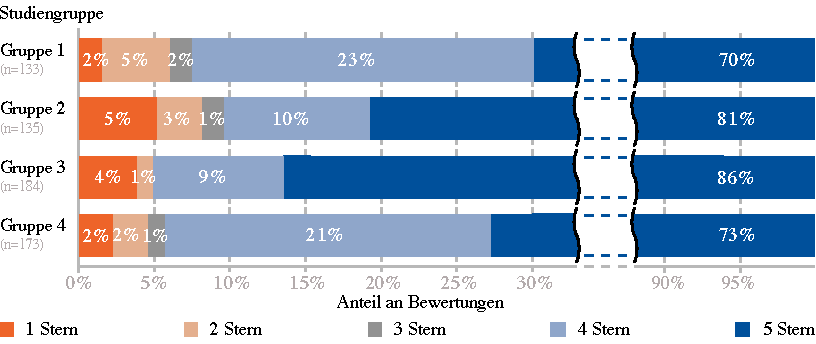
\includegraphics[width=\linewidth]{contents/06_model_evaluation/02_evaluation/res/rating_result_overview.pdf}
    \caption{Verteilung der Teilnehmer-Bewertung der Navigation für jede Studiengruppe bezogen auf die insgesamt abgegebenen Bewertungen}
    \label{fig:Rating_Result_Overview}
\end{figure}

Für die Prüfung zwischen welchen Studiengruppen ein signifikanter Unterschied vorliegt, wird wieder der Dunn-Test \cite{dunn1964multiple} verwendet, nachdem ein Kruskal-Wallis-Test einen Haupteffekt zeigt ($ p = 0.00335 $). Daraus resultiert, dass es zwischen den Gruppen 1 und 3 ($ p = 0.005723$) sowie 3 und 4 ($ p = 0.024375 $) einen signifikanten Unterschied bei der Zufriedenheit mit der aktuellen Route gibt. Mithilfe von \autoref{fig:Rating_Result_Overview} wird abgeleitet, dass es insbesondere mehr 5-Stern-Bewertungen in Gruppe 3 gegenüber den Gruppen 1 und 4 gibt. Die Anteile der ein und zwei Stern Bewertungen unterscheiden sich kaum. Folglich kann man sagen, dass die Teilnehmer signifikant zufriedener mit der Navigation waren, wenn sie Erklärungen wie in Gruppe 3 bekommen im Vergleich zu keinen Erklärungen (Gruppe 1) oder allen vorgestellten Erklärungstypen (Gruppe 4).

Da beim Geben von Erklärungen dies die Nutzerzufriedenheit nicht in jedem Fall erhöht, muss Hypothese 3.1 abgelehnt werden. Hypothese 3.2 muss ebenfalls abgelehnt werden, unter anderem da es einen gegenteiligen Effekt zwischen den Gruppen 3 und 4 gibt.

\subsubsection{Häufigkeit der Nutzung}
\label{sec:06_model_evaluation:usage_analysis}

Bei der Analyse der Nutzungshäufigkeit von NUNAV wird über den zweiwöchigen Studienzeitrum geprüft, wie viele Routen pro Nutzer und Studiengruppe in diesem Zeitraum gefahren wurden.

\textbf{Hypothesen}

\begin{enumerate}
    \item[4.1] WENN Teilnehmer Erklärungen erhalten, DANN verwenden sie NUNAV signifikant häufiger, als wenn sie keine erhalten.
    \item[4.2] WENN Teilnehmer nur einen der beiden vorgestellten Erklärungstypen erhalten, DANN nutzen sie NUNAV signifikant seltener, als wenn sie beide Erklärungstypen erhalten.
\end{enumerate}

Bei der Betrachtung der Anzahl der gefahrenen Routen werden die Daten zunächst normalisiert. Folglich sind 3 951 Nutzer im Datensatz für die Prüfung der Hypothesen verblieben.

\begin{figure}
    \centering
    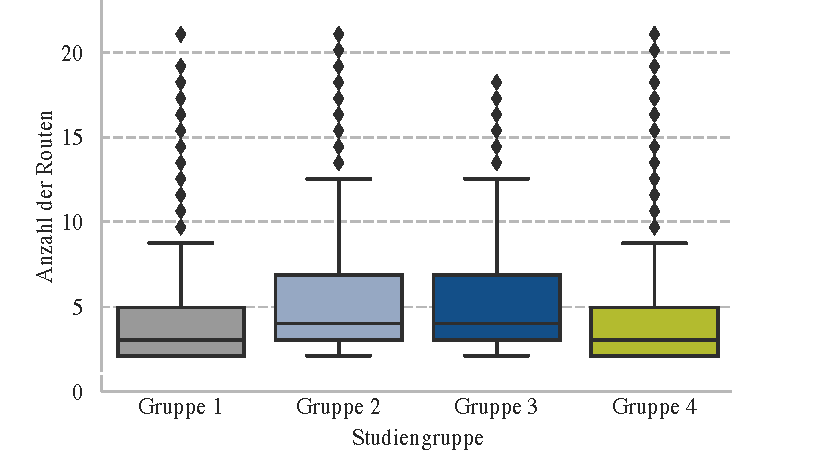
\includegraphics[width=\textwidth]{contents/06_model_evaluation/02_evaluation/res/usage_result_overview.pdf}
    \caption{Anzahl der gefahrenen Routen für jede Studiengruppe}
\end{figure}

\begin{table}
    \centering
    \begin{tabular}{|c|c|c|c|}
        \hline
        \textbf{Studiengruppe}  & \textbf{Mittelwert} [N] & \textbf{Standardabweichung} [N] \\ \hline
        Gruppe 1                & 3.2672 & 3.2958 \\ \hline
        Gruppe 2                & 3.2256 & 3.1961 \\ \hline
        Gruppe 3                & 4.6630 & 4.7043 \\ \hline
        Gruppe 4                & 4.5391 & 4.1509 \\ \hline
    \end{tabular}
    \caption{Übersicht der Ergebnisse der gefahrenen Routen der Nutzer}
    \label{tab:study_offroute_results_2}
\end{table}

Zur Prüfung der Signifikanz wird wieder der Kruskal-Wallis-Test eingesetzt, da auch die Daten der Anzahl der gefahrenen Routen pro Studienteilnehmer nicht normalverteilt sind (Shapiro-Wilk: $ p = 0.0000 < 0.05 $). Mit $ p = 1.146748e-16 $ kann davon ausgegangen werden, dass ein Haupteffekt vorliegt.

Für die Prüfung zwischen welchen Studiengruppen ein signifikanter Unterschied vorliegt, wird auch hier der Dunn-Test verwendnet. Die Prüfung ergibt, dass jeweils ein signifikanter Effekt zwischen den Gruppen 3 und 4 gegenüber den Gruppen 1 und 2 vorliegt. Folglich kann abgeleitet werden, dass die Nutzer NUNAV häufiger verwenden, wenn sie die Erklärungen während der Navigation erhalten unabhängig davon, ob diese kombiniert mit den Erklärungen vor der Navigation erfolgen.

Die Hypothesen 4.1 und 4.2 müssen abgelehnt werden, da weder alle Erklärungstypen zu einer signifikant häufigeren Nutzung von NUNAV führen, noch das Geben von beiden vorgestellten Typen von Erklärungen zu einer erhöhten Nutzung pro Studienteilnehmer führt im Vergleich zur Präsentation von nur einem der integrierten Erklärungstypen.

\subsubsection{Bedarf für die gegebenen Erklärungen}

Die statischen Erklärungen (siehe \autoref{sec:user_count_definition} und \autoref{sec:route_explanation_definition}), welche die Einflüsse auf den Routing-Algorithmus von NUNAV sowie das kollaborative Routing erklären, sind interaktiv. Somit kann evaluiert werden, wie viele Studienteilnehmer wie häufig diese angefordert haben. Außerdem kann gemessen werden, wie lange sie die Erklärungen betrachtet haben.

Die drei verschiedenen Erklärungen, die die Nutzer aufrufen können, sind in \autoref{sec:user_count_definition} und \autoref{sec:route_explanation_definition} beschrieben. Die Studiengruppen (Gruppe 2 und 4), denen diese angezeigt wurden enthalten insgesamt 1 766 Teilnehmer.

Im Folgenden wird die Erklärung zum Routing-Algorithmus \textit{Erklärung 1}, die kurze Erklärung zum kollaborativen Routing als \textit{Erklärung 2} und die dazugehörige weitere Erklärung als \textit{Erklärung 3} genannt.

Als gelesen bzw. zumindest entschieden, ob die Erklärung benötigt wird gilt diese, wenn ein Nutzer länger als 1,5 Sekunden in dem Dialog verbracht hat \cite{BAHR2011776}. \autoref{fig:explanation_results_clicked} zeigt wie häufig die Nutzer eine Erklärung angefordert haben und diese auch zumindest zum Teil gelesen haben. \autoref{tab:explanation_results_clicked} zeigt die Bewertung als \glqq Hilfreich\grqq{} oder \glqq Nicht hilfreich\grqq{} durch die Nutzer. Allerdings sind die Hilfe-Artikel auch über andere Wege erreichbar, wodurch Bewertungen nicht nur von Nutzern kommen, die über die NUNAV-App dort hingeleitet wurden.

\begin{figure}
    \centering
    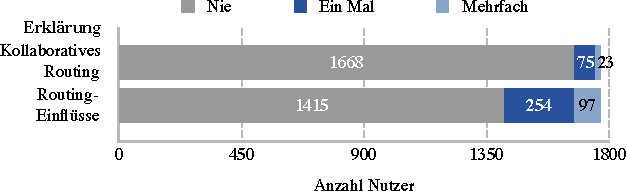
\includegraphics[width=\linewidth]{contents/06_model_evaluation/02_evaluation/res/explanation_results_clicked.pdf}
    \caption{Häufigkeit des Anforderns der Erklärungen pro Nutzer}
    \label{fig:explanation_results_clicked}
\end{figure}

\begin{figure}
    \centering
    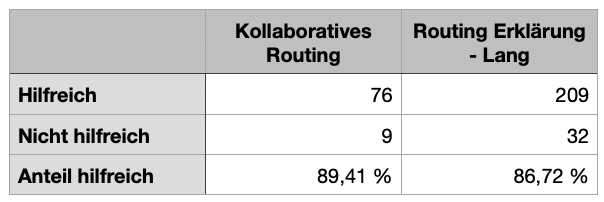
\includegraphics[width=\linewidth]{contents/06_model_evaluation/res/explanation_results_clicked_support.png}
    \caption{Bewertung der langen Erklärungen (Support-Artikel)}
    \label{tab:explanation_results_clicked}
\end{figure}

\subsubsection{Zusammenfassung}

% \begin{figure}
%     \text{Evaluation des Erklärungsbedarfs} \\
%     \subfloat[Anzahl der Teilnehmer, die Erklärung 1 angefordert haben]
%     {\includegraphics[width=.3\linewidth]{contents/06_model_evaluation/res/evaluation_explanation_1_clicks.pdf}}
%     \hspace{5mm}
%     \subfloat[Anzahl der Teilnehmer, die Erklärung 2 angefordert haben]
%     {\includegraphics[width=.3\linewidth]{contents/06_model_evaluation/res/evaluation_explanation_1_clicks.pdf}}
%     \hspace{5mm}
%     \subfloat[Anzahl der Teilnehmer, die Erklärung 2 angefordert haben]
%     {\includegraphics[width=.3\linewidth]{contents/06_model_evaluation/res/evaluation_explanation_1_clicks.pdf}} \\
%     \subfloat[Berechnete und reale Koordinaten]
%     {\includegraphics[width=.47\linewidth]{gfx/MagnetEvaluation/alg1-n48/grafic3.pdf}}
%     \hspace{5mm}
%     \subfloat[Relativer Rechenfehler]
%     {\includegraphics[width=.47\linewidth]{gfx/MagnetEvaluation/alg1-n48/grafic4.pdf}}
%     \caption[Evaluation der Positionsbestimmung mithilfe des Coulombschen Gesetzes]{Evaluation der Positionsbestimmung mithilfe des Coulombschen Gesetzes bei Verwendung eines Magneten mit Magnetisierungsgrad N48, 8 mm Durchmesser und 20 mm Länge}
%     \label{fig:evaluation_explanations_clicks}
% \end{figure}

Keinen Zusammenhang zwischen den Erklärungen und einer schlechteren / späteren ATA

\subsubsection{Qualitativ}
\label{sec:study_results_qualitativ}